% !TeX program = lualatex
\documentclass[a4paper,12pt,twoside]{article}
\usepackage{rhreport}

\begin{document}
\thispagestyle{empty}
%\tikz[remember picture,overlay][t!] \node[opacity=3,inner sep=2pt] at (current page.center){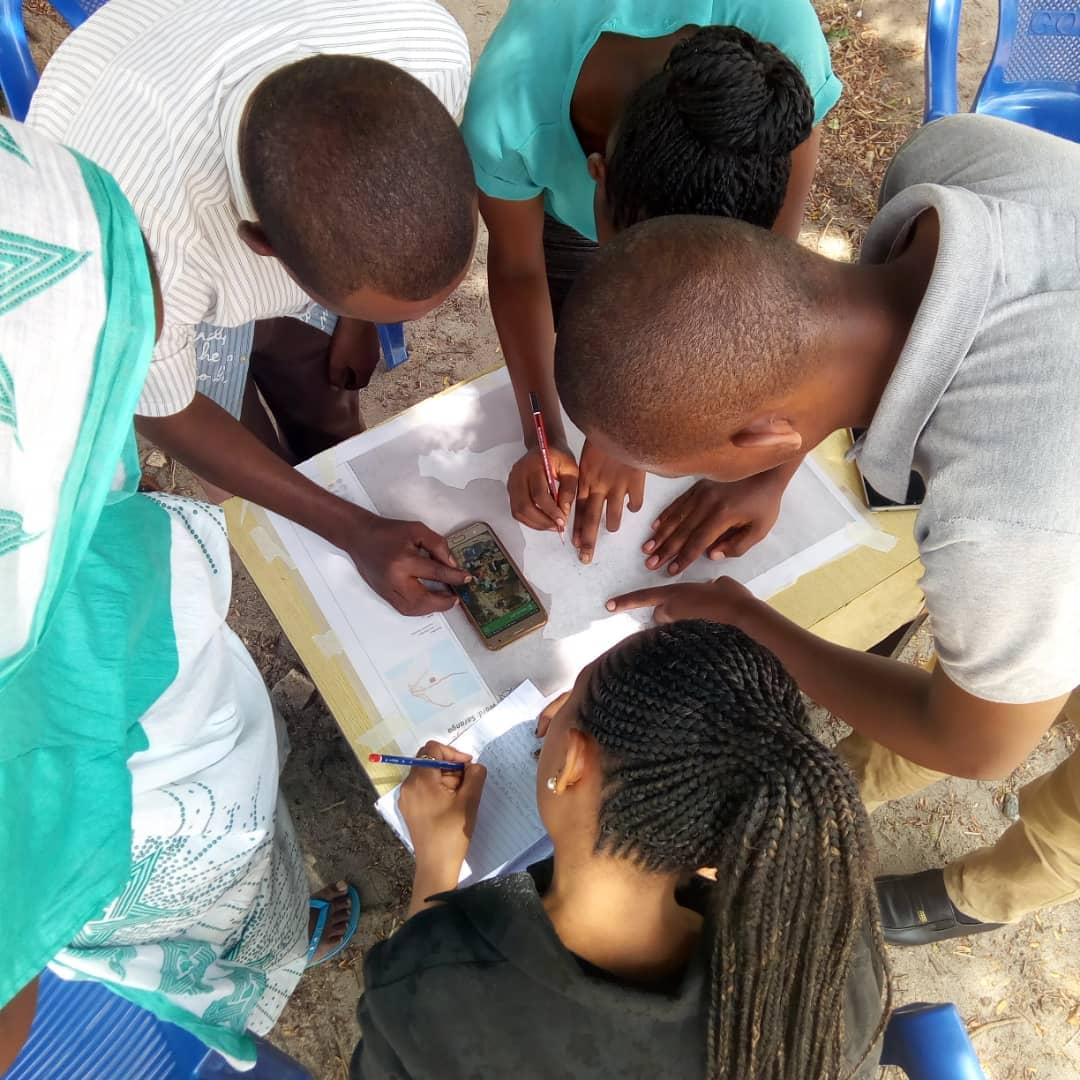
\includegraphics[width=\paperwidth,height=\paperheight,keepaspectratio]{images/RHcoverphoto.jpg}};
%\clearpage


\begin{figure}[t!]
\centering
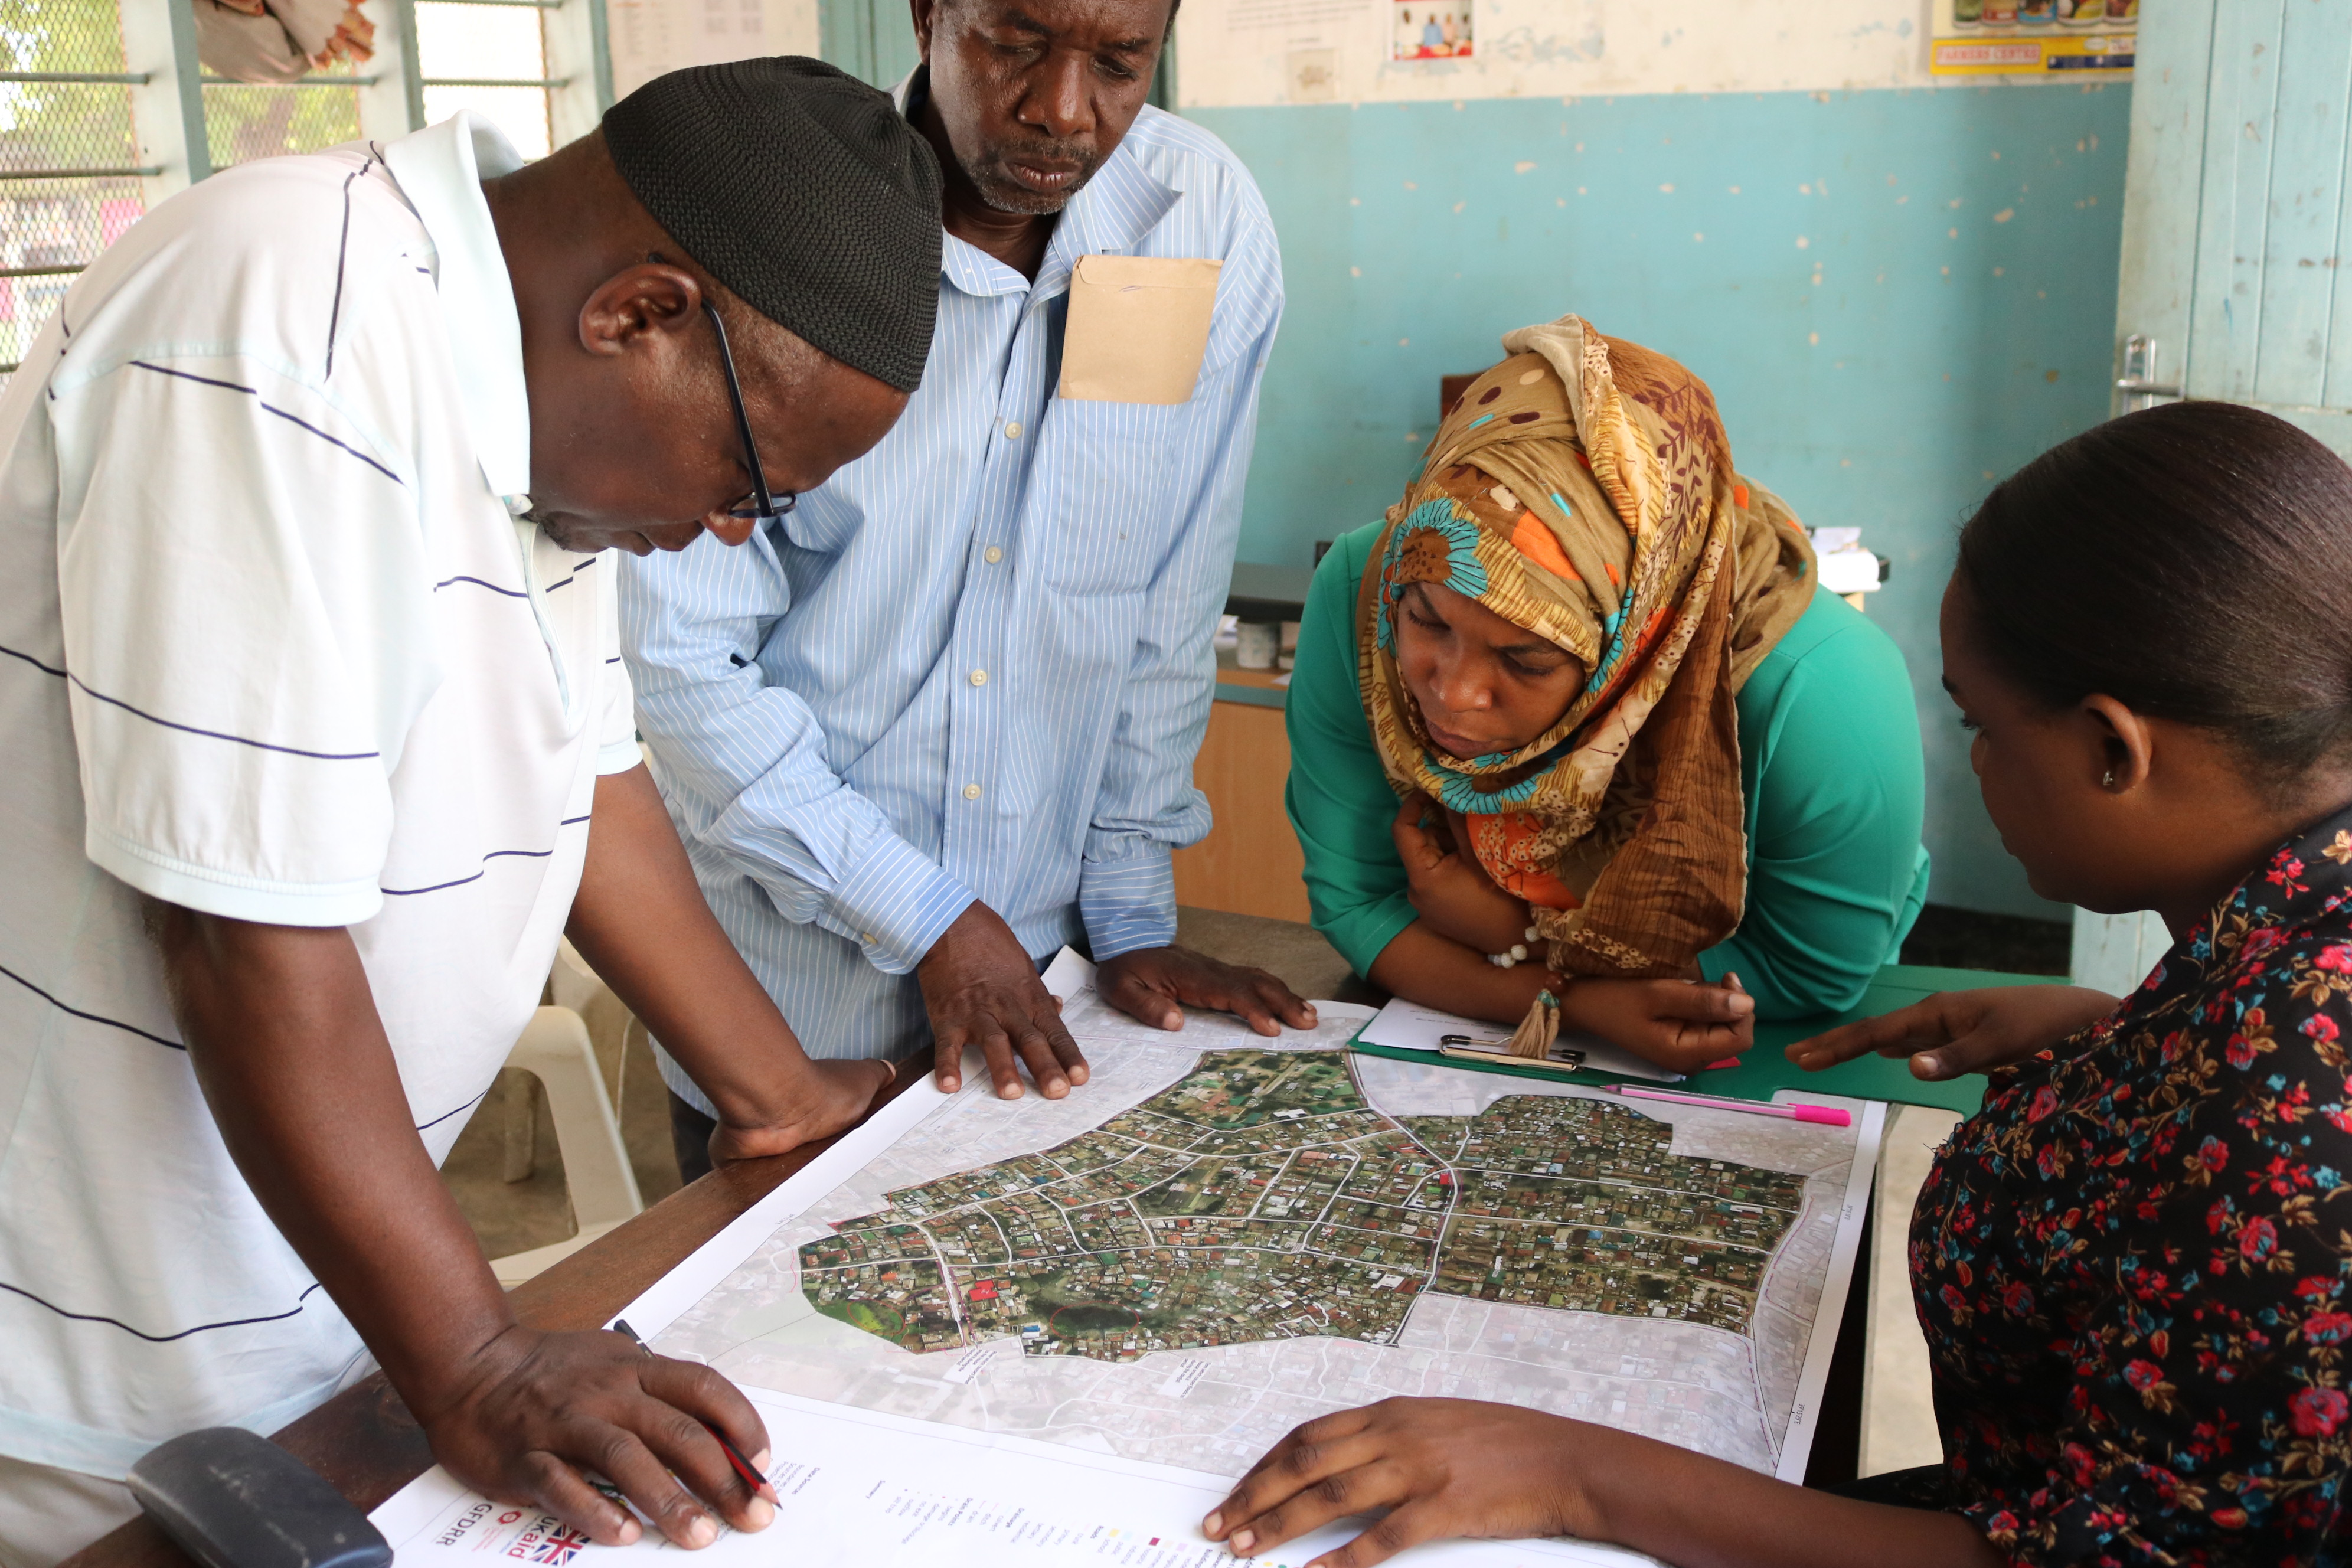
\includegraphics[width=\textwidth, height=12cm]{images/CommunityMeeting_Sia.JPG}
\end{figure}


%\begin{center}
%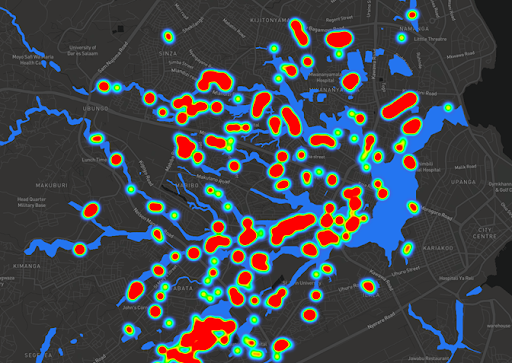
\includegraphics[width=\textwidth]{images/Asset_&_Threats_Viz.png}
%\end{center}
\begin{center}
  \huge \color{RHblue} \textbf {RAMANI HURIA}

\textbf{FINAL REPORT}
\end{center}
\medskip
\vbox{
  \centering
  Prepared for:
  \vcenteredhbox{
\includegraphics[width=2cm]{UK-aid_logo.png}}
  and { }
  \vcenteredhbox{
\includegraphics[width=7cm]{images/World_Bank_Group_logo.png}}
  \
  
  by:
  \vcenteredhbox{
\includegraphics[width=4cm]{HOT_logo_with_text.png}}
  % \maketitle
  
}

\begin{center}
  Humanitarian OpenStreetMap Team
  \
  
  September, 2019
\end{center}
\medskip
\begin{center}
\color{RHblue}\rule{\textwidth}{0.5cm}
\end{center}

\newpage
\color{RHgrey}

\begin{center}
{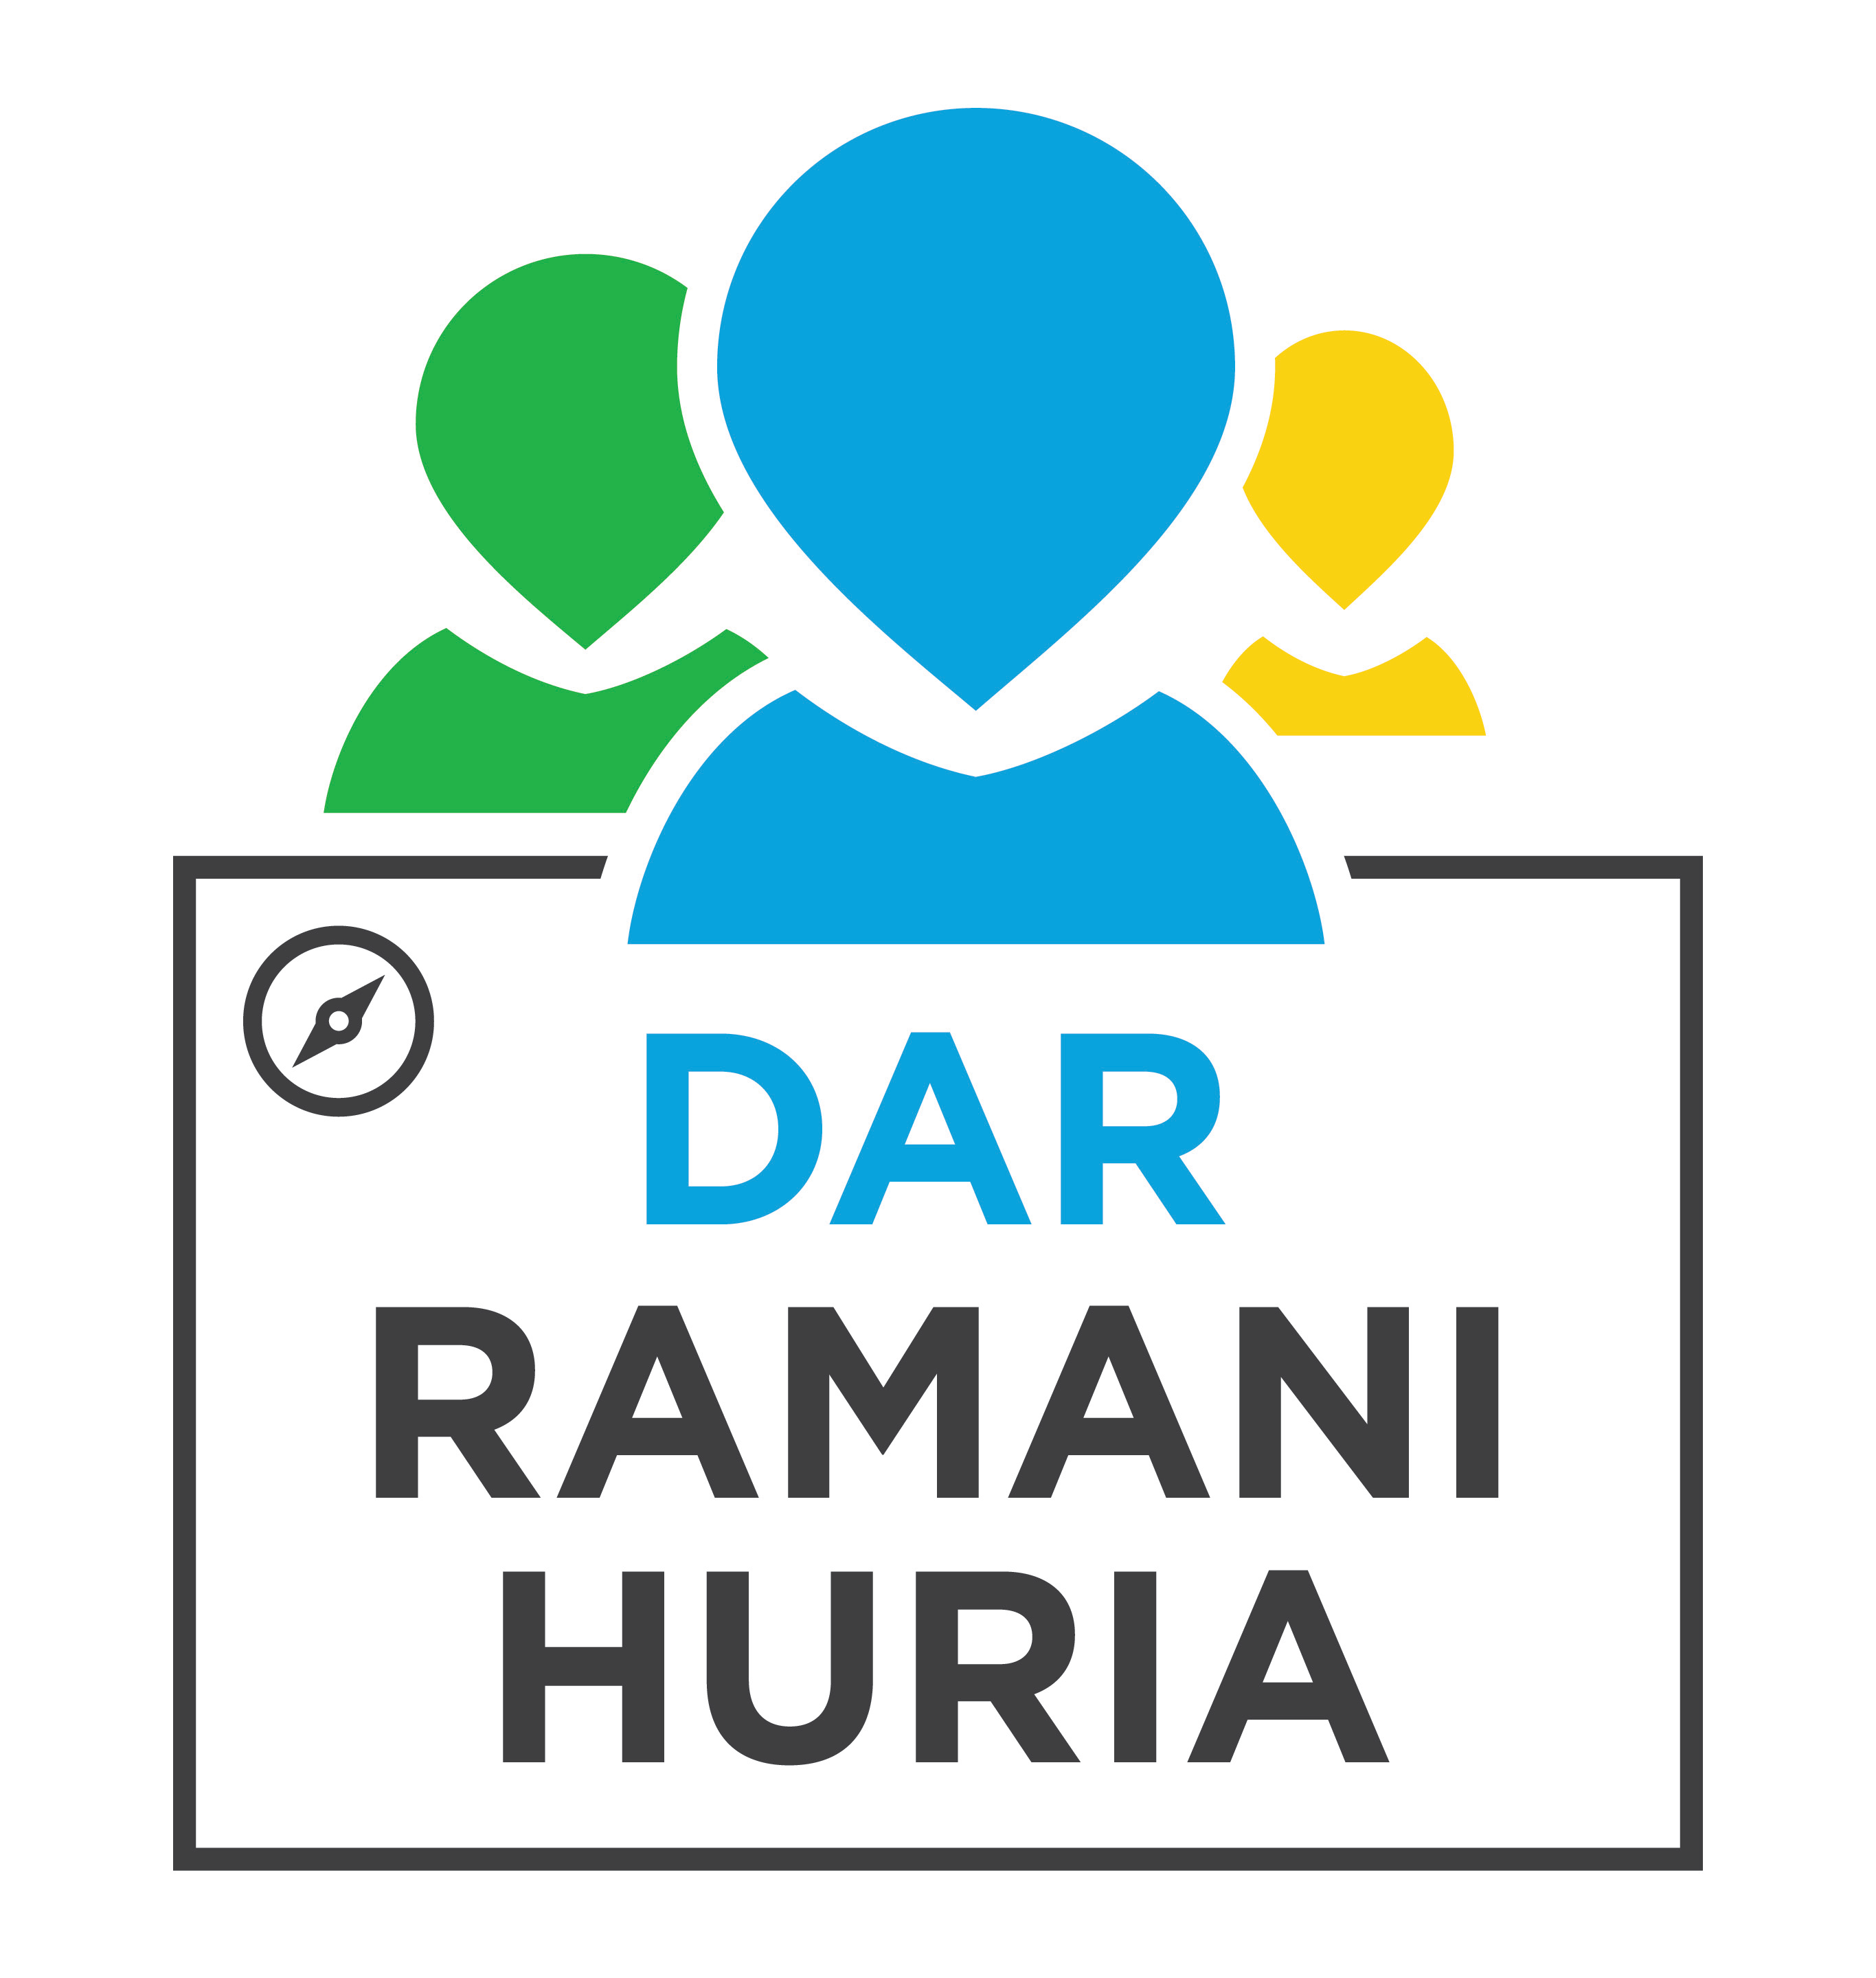
\includegraphics[width=5cm]{Dar_Ramani_Huria_logo.png}}
\end{center}

This report was prepared by Immaculate Mwanja, Hawa Adinani, Innocent Maholi, William Evans, Ivan Buendia Gayton, Jess Beutler, Paul Uithol, Iddy Chazua, Asha Mustapher, Godfrey Kassano, Elia Dominic, Tyler Radford and many others from the Humanitarian OpenStreetMap Team in Tanzania.

Graphic design by Ivan Buendia Gayton and Immaculate Mwanja based on the Ramani Huria design guideline by Darragh Amelia Coward. Layout was done using the \LaTeX{} typesetting system.

Guidance and input on the project came from Edward Anderson, Caroline Gevaert, Roza Vasileva, Darragh Amelia Coward and Msilikale Msilanga at the World Bank.

Unless otherwise noted, photos by the Ramani Huria team. Maps were prepared by the Ramani Huria team using QGIS.


\bigskip\bigskip\bigskip\bigskip\bigskip

\begin{center}
\vcenteredhbox{
\includegraphics[height=2cm]{images/logo_Coat_of_arms_of_Tanzania.png}}
\vcenteredhbox{
\includegraphics[height=2.2cm]{UK-aid_logo.png}}
\vcenteredhbox{
\includegraphics[height=1.2cm]{images/World_Bank_Group_logo.png}}
\vcenteredhbox{
\includegraphics[height=0.7cm]{images/logo_GFDRR.png}}

\medskip

\vcenteredhbox{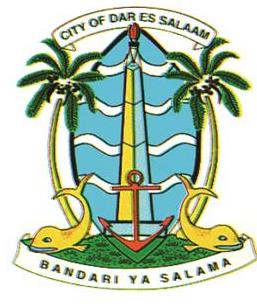
\includegraphics[height=1.2cm]{images/logo_dar-es-salaam.jpg}}
\vcenteredhbox{
\includegraphics[height=1.2cm]{images/logo_Ardhi.png}}
\vcenteredhbox{
\includegraphics[height=1.2cm]{images/logo_costech.png}}
\vcenteredhbox{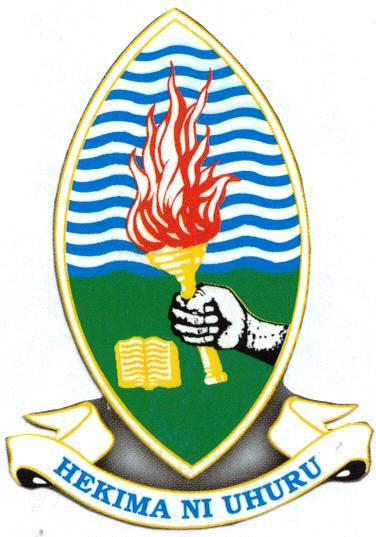
\includegraphics[height=1.2cm]{images/logo_UDSM.jpg}}

\end{center}

\newpage

% Reduce the spacing between Table of Contents items to get it down to 1 page

\renewcommand{\baselinestretch}{1.0}\normalsize
\tableofcontents
\renewcommand{\baselinestretch}{1.0}\normalsize

\newpage

\setlength{\parskip}{0.4em}
\section{Foreword}
\begin{multicols}{2}
In early 2015, I had the pleasure of getting to know a group of enthusiastic students from Ardhi University and the University of Dar es Salaam. This group of young people were given a challenging assignment: Create digital and print maps of each and every flood-prone ward of Dar es Salaam, and train community members living in the most flood prone and least developed wards to take part. And do it all in a few months during school break. This was no easy feat: The best available public maps had not been updated in many years and could simply not keep up with the dramatic urbanization of one of Africa’s fastest growing cities.
 
What I observed during each trip to Dar es Salaam from 2015-2018 was remarkable. Students and community members, many of whom had experienced flooding in their own homes, transformed themselves from passive survivors of disaster to active resilience builders by identifying key infrastructure and flood-prone areas of their city. The team learned to fly drones, much to the excitement of nearby schoolchildren, capturing photos of high risk wards at lower cost and higher resolution than any commercial satellite anywhere in the world. Students motivated community members, most of whom did not have experience using a smartphone or laptop. As the team held community workshops in each ward you could often hear them chanting “Ramani HURIA!”.
 
Bit by bit, the invisible became visible: entire wards, home to tens of thousands of people, lit up on OpenStreetMap with the incredible complexity that exists in unplanned neighborhoods. And over time, I was fortunate enough to witness the scrappy student interns mature into some of the continent’s most skilled and capable digital mapping experts. Over 1 million buildings – each and every building in Dar es Salaam – became part of the map. Students became project leaders, gaining skills which led to employment both with the project team and with the government of Tanzania. Skills and methodology developed by the project enabled community-led responses to the 2016 earthquake in Bukoba and episodes of heavy flooding in Dar es Salaam. Other innovations followed in later years: soil sediment sampling and a drone built from local materials, which enabled mapping the city’s solid waste disposal challenge and major river basins.
 
Ramani Huria has been highlighted as a model of community-led resilience by the IFRC 2018 \textit{World Disasters Report,} the International Institute for Sustainable Development (IISD) report Big Data for Resilience Building, the Sustainable Development Solutions Network (SDSN) TReNDS report \textit{“Counting on the World”} as well as a number of other publications. The data contributed by students and community members is now serving as input to Silicon Valley’s top AI and machine learning models that have the potential to fill map data gaps for entire countries on the African continent. As the project draws to a close, what I’m most hopeful for is the “ripple effect”. The changes in the trajectory of students’ lives have been incredible due to their participation in the project. I can only imagine the possibilities for the data and awareness generated by the project to be put to use in new and unexpected ways; positively affecting the lives of the city’s inhabitants in the years to come.
\end{multicols}

--Tyler Radford, \textit{Executive Director}, Humanitarian OpenStreetMap Team (HOT)
\clearpage

\newpage
\section{Executive Summary}
\label{executivesummary}
%\begin{multicols}{2}

Ramani Huria is a community-based mapping project in Tanzania that began in 2015, training university students and community members to create accurate maps of the most flood-prone areas of Dar es Salaam. 

One of the fastest-growing cities in Africa, Dar es Salaam is projected to become a mega city of over 10 million people in the next six years. In addition to this dramatic growth, more than 70 percent of the city's residents live in informal, unplanned settlements that lack basic infrastructure and services. Rising temperatures, longer dry spells and more intense heavy rainfall have made Tanzania the most flood-affected country in East Africa.

The Government of Tanzania has recognized these risks, and is taking proactive and preventive actions to build resilience to minimize the economic and human cost of disaster. In partnership with the United Kingdom's Department for International Development and the World Bank, the Tanzania Urban Resilience Program (TURP) was established to coordinate strategic action for preparing, responding, and adapting to a changing climate.

Three core challenges were identified, namely a lack of data and information, an inadequate urban and land use planning system, and significant infrastructure gaps. To address these, a multi-sector approach was designed based around three pillars: Risk Identification, Risk Reduction, and Disaster Preparedness and Emergency Management. 

The Humanitarian OpenStreetMap Team (HOT) was selected  to help implement  Ramani Huria. As the world's preeminent participatory mapping organization, HOT emphasizes training local people  to develop their own capacity to understand and respond to risk. The strategic significance of this is threefold: 

\begin{itemize}
    \item First, by empowering Tanzanian citizens and leaders, Ramani Huria invests in local people to reach a depth of understanding that would otherwise be impossible to achieve. Local communities possess expert knowledge of their environments and are best prepared to represent and own their own data. 
    \item Second, traditional surveying and Geographical Information Systems (GIS) are often costly and dependent on proprietary software. In contrast, Ramani Huria has deployed open source tools to combination with local devices to ensure that cost is not a barrier to quality work.  
    \item Third, in documenting the project every step of the way, the team is creating open knowledge that will be a readily available resource to others looking for a way forward. It is thus a longstanding resource, in the spirit of open-source projects. 
\end{itemize}

The impact of what has been accomplished far surpasses what would have otherwise been possible using other methods. At times the project has swelled to involve hundreds of university students, and thousands of community members, with a geographic reach across the city. We are  the largest community mapping initiative in Africa.
 
%\end{multicols}

\newpage
\section{Introduction}
\label{Introduction}
\begin{multicols} {2}

The story of Ramani Huria begins with a flood. In 2011 Tanzania experienced the heaviest rains since independence in 1961 - leading to widespread devastation of infrastructure, thousands of displaced people, and a significant loss of life. 

The 2011 floods were a wakeup call, and soon thereafter it was recognized that the status quo was unacceptable. Experts agreed that the flooding was not just a natural phenomenon, but rather man-made—a direct result of development. Efforts were soon underway to research the best practice from other cities. 

The Tanzanian Government made a request through the Commission of Science and Technology (COSTECH), to support a better approach to addressing the floods. Any viable solution needed to be both local and sustainable. In response, the World Bank supported a community-based flood mapping innovation.

After initial success from 2015-2016, the Tanzanian Ministry of Lands and Regional Administrative Secretary of Dar es Salaam requested an extension, to promote flood resilience and student skills. Under the TURP framework, the World Bank signed a Memorandum of Understanding with Ardhi University in September of 2017, laying the foundation for a Resilience Academy —Ramani Huria being its first major project.

The team was initially built from graduates of local universities, most of whom had backgrounds in Urban Planning and Geography. They themselves were new to open source tools and the participatory mapping process, and yet were eager to develop these skills. One of the first major undertakings was coordinating the Industrial Training in 2017, a practical two-month internship for university students to gain real world experience. 

In addition to trainings on various mapping tools, 2017  involved a lot of digitization - primarily tracing buildings and roads to create a basemap of the city. This proved for the first time  that it is possible to run efficient large-scale digitization using African mobile internet connections. Many of the students continued to work by conducting individual household surveys focused on historical flood extents. Finally, towards the end of the year, the team obtained its official registration as a local non-governmental organization called OpenMap Development Tanzania (OMDTZ). 

2018 began with an important week-long workshop that brought together over 40 stakeholders including government, civil society, academia, communities, and local authorities. Participants were introduced to Ramani Huria’s work, data, and tools, while seeds were sown for impactful data use. Another key event of this year was the Msimbazi Charrette, an urban design process that drew on the views and experiences of diverse stakeholders who envision a more resilient basin. Ramani Huria assisted this process by extending the surveys in support of the charrette. Data collection continued across the city, with extensive surveys being conducted to build important layers of assets, trash points, and hyperlocal boundaries. 

In 2019, the original cohort of young graduates looked more like a professional team with expertise in data collection, quality assurance using GIS, and community engagement. The activities conducted during the final year involved a soil sediment profile of the city, two community flood responses following heavy rainfalls, and aerial imagery of the main rivers and solid waste of Dar es Salaam with drones. 

As the project draws to a close, a great effort has been made to hand over both resources and responsibilities to the Resilience Academy, an initiative led by dedicated faculty of five academic institutions: Ardhi University (Tanzania), University of Dar es Salaam (Tanzania), Sokoine University of Agriculture (Tanzania), State University of Zanzibar (Zanzibar), and University of Turku (Finland). They inherit the legacy of Ramani Huria, and will ensure that its achievements are passed on to Tanzania’s future leaders. 

This report showcases the work done from July 2017 to August 2019, highlighting partners, datasets, major activities, lessons learned, ongoing and future impacts, and why other cities and countries around the world should consider adapting Ramani Huria as a model for resilience.

\end{multicols}

\section{Partners}
\begin{multicols}
\medskip
\textbf{Ardhi University -} One of Ramani Huria’s primary partners, Ardhi University is a public university in Dar es Salaam, Tanzania, with an expertise in land studies. Ardhi places hundreds of students for the Industrial Training and many of the Ramani Huria team are graduates of the university

\textbf{Commission of Science and Technology (COSTECH) -} COSTECH is responsible for supporting research and development activities across Tanzania within the technology sector. Ramani Huria liaises with COSTECH for training, official contacts, and data sharing.

\textbf{Dar es Salaam City Council -} Dar es Salaam City Council governs Tanzania’s economic capital. They are a key partner and help provide authorization for activities throughout Dar es Salaam. 

\textbf{Dar es Salaam Metropolitan Development Project (DMDP) -} Dar es Salaam Metropolitan Development Project aims to improve urban services and institutional capacity in the metropolitan area and to facilitate emergency response. As a responsible party for financing improvements and constructions of infrastructure, they benefit from the diverse datasets of Ramani Huria. 
\

\textbf{Delft University of Technology - Water Resources Management (TU Delft) -} Housed within the largest and oldest Dutch public technological universities, TU Delft's Water Management Department is currently establishing a hydrometeorological observation network under TURP, as part of the Trans-African Hydro-Meteorological Observatory (TAHMO). TU Delft is collaborating with HOT and Deltares to assess if their monitoring stations, in combination with low-cost roving barometer sensors, can be used to measure elevation, relative to the TAHMO station's position. TU Delft is facilitating this research through students’ exchange. 

\textbf{Deltares -} An independent institute for applied research in the field of water, Deltares works with HOT on the data quality assurance of drainage data, as well as supervising students to pilot using the data in hydraulic modeling of water transport and flooding. 

\textbf{Department for International Development (DFID) -} The main donor of the Ramani Huria initiative providing funding through the Tanzania Urban Resilience Program, a partnership between the United Kingdom’s Department for International Development (DFID) and the World Bank established to support the Government of Tanzania in its endeavor to increase resilience to climate and disaster risk. 
\textbf{Tanzania Data Lab (dLab) -} The Tanzanian Data Lab (dLab) is an open working space where data from multiple sectors and sources can be combined, processed, and shared to drive better policies and decision-making. 

\

\textbf{Global Facility for Disaster Reduction and Recovery (GFDRR) -} The World Bank’s Global Facility for Disaster Reduction and Recovery (GFDRR) is a global partnership that helps developing countries better understand and reduce their vulnerabilities to natural hazards and adapt to climate change. GFDRR has provided significant support since the beginning of the Ramani Huria initiative.

\

\textbf{The Government of Tanzania (GoT) -} The Government of Tanzania is an implementing partner of the Ramani Huria project and has been supporting the initiative since 2015. We have been working with five municipalities in Dar es Salaam to make sure they are aware of the project and its potentialities. Key government agency partners include the President’s Office for Regional and Local Government (PORALG), Disaster Management Department (DMD), National Bureau of Statistics (NBS), Tanzania Meteorological Agency (TMA).

\

\textbf{Tanzania Red Cross Society (TRCS) -} The Tanzania Red Cross Society (TRCS) is a voluntary and independent humanitarian organization that joined the worldwide network of Red Cross and Red Crescent Societies in 1963. TRCS aims to mobilize resources through the power of humanity towards improving the situation of the most vulnerable in Tanzania. During the 2018 Industrial Training, TRCS volunteers worked together with RH teams and community members to build the community asset and threat inventories.

\textbf{University of Dar es Salaam (UDSM) -} The University of Dar es Salaam is the oldest and largest public university in Tanzania, established on 1st July 1970. UDSM is a member of the Resilience Academy and has contributed students to Ramani Huria Industrial Trainings. 

\textbf{University of Twente -} The University of Twente in the Netherlands is the author of the Ramani Huria Cookbook for academic partners to make use of the methods, protocols, and learnings of the project. This is intended to help post-secondary educational institutions prepare their students for participation in community mapping projects. 

\textbf{World Bank -} The World Bank is the funder of the Ramani Huria project. Ramani Huria activities form part of the Tanzania Urban Resilience Programme, a partnership between the World Bank and the United Kingdom’s Department for International Development (DFID).
\end{multicols}

\newpage
\section{Datasets}

\subsection{Summary of Datasets Collected}
\begin{multicols}{2}


Ramani Huria organized a series of community mapping campaigns collecting geospatial data on infrastructure and exposure to risk. These activities played a vital role in engaging communities, strengthening resilience, and enabling data-driven planning and preparedness for disasters. 
For training purposes, community mapping teams collected a variety of data sets including points of interest, location of businesses, schools, and hospitals,  and local knowledge on flooding that might be of interest to various audiences.
The Ramani Huria datasets are broken down by three separate components—Exposure, Environment, Hazard—under TURP. Much of the data is contributed by communities and users of \href{https://www.openstreetmap.org/}{OpenStreetMap}\footnote{\url{https://www.openstreetmap.org/}}; including students and community members. For a comprehensive list of these datasets, please reference the Climate Risk Database hosted by the \href{https://geonode.resilienceacademy.ac.tz/}{Resilience Academy GeoNode}\footnote{\url{https://geonode.resilienceacademy.ac.tz/}} or refer to the Technical Overview of Digital Assets listed as an annex.

Ramani Huria teams collected and created a wide range of base map data—over 20 geospatial datasets for Dar es Salaam—which primarily sit on the OpenStreetMap platform under the Open Data Commons Open Database License (ODbL) license. This is the underlying map layer upon which specific datasets important to resilience are overlaid—the equivalent of common web-based maps such as Google Maps, but freely available open data backed by a global community and extensive quality assurance.
This includes roads, buildings, health care facilities, schools and universities, transportation infrastructure such as bus stops and Rapid Transit lines, businesses such as restaurants, shops, salons and hotels, public offices, recreation facilities, natural features such as rivers and wetlands, parks, etc. This data is being constantly updated as the physical features of the city change and evolve, as well as when users or the community choose to focus on a particular feature type (for example, if a local agency wishes to visualize where people get drinking water, volunteers—including Ramani Huria students—may specifically focus on features relevant to that need for a time.
Besides base data, other major digital assets that were collected in the Ramani Huria project include drainage data, soil sediment sampling, community assets & threats, building footprint re-digitization, hyperlocal administrative boundary, trash mapping, community flood response, and historical flood extents. All of these datasets except the building footprint re-digitization are under the \href{https://creativecommons.org/licenses/by/4.0/}{Creative Commons (CC-BY 4.0)}\footnote{\url{https://creativecommons.org/licenses/by/4.0/}} license enabling the free distribution of an otherwise copyrighted work.
OpenStreetMap is a global map! There is no particular boundary or extent to this data. However, the team’s efforts are focused on greater Dar es Salaam, with a particular focus on the 46 prioritized Ramani Huria wards (just under 50 percent of the wards in the city).
\end{multicols}

\subsection{Data Collection Methodology}
Ramani Huria base data was collected and created using a range of tools in the OpenStreetMap and Humanitarian OpenStreetMap Team ecosystem, including but not limited to the Java OpenStreetMap Editor (JOSM), OpenDataKit, OpenMapKit, iD Editor, HOT Tasking Manager, and QGIS. 
The two main categories of data creation are remote mapping and field mapping. Remote mapping is done using aerial or satellite imagery, usually with the JOSM tool, a desktop editing software that provides a comprehensive suite of tools for viewing imagery and creating vector features over the raster background. Ramani Huria teams, alongside global OpenStreetMap volunteers, have digitized every feature visible in aerial imagery of the greater Dar es Salaam city, including over one million individual buildings and virtually all roads.
Field mapping, usually using OpenDataKit or its derivative OpenMapKit, involves physically visiting features to add local information such as road names, building type, amenities, etc.

\subsection{Data Quality}

Data quality assurance is the process of data profiling to discover inconsistencies and other anomalies in the data, as well as performing data cleaning activities (e.g. removing outliers, missing data interpolation) to improve the data quality. Data description is done using descriptive statistics; these are used to describe the basic features of the data in a study. They provide simple summaries about the sample and the measures. Together with simple graphics analysis, they form the basis of virtually every quantitative analysis of data.
Data quality activities involve data rationalization and validation. Ramani Huria's activities follow the HOT Data Quality Framework as a guide for each dataset to ensure the data is cleaned following certain procedures and steps. The objective of the framework is to provide insight into the data quality process as well as to guide future projects in best practices. See \href{https://docs.google.com/document/d/1IE1ARLs6i4d_KTK73X9LGbU2OoEHCgDRefE47J6LJn8/edit#}{HOT Data Quality Framework.}\footnote{\url{https://docs.google.com/document/d/1IE1ARLs6i4d_KTK73X9LGbU2OoEHCgDRefE47J6LJn8/edit#}}
Data that have been uploaded to OpenStreetMap have a clearly defined data model. Ramani Huria teams use tools such as OSMCHA, JOSM, QA, Osmose, KeepRight, and GIS utilities to ensure that Ramani Huria data conforms to the data model and contains minimum errors.

\subsection{Human Resources Deployed}

Ramani Huria teams were formed from university students, who originally digitized base data from aerial or satellite imagery.  As time went on, these students became mapping  supervisors who taught and mentored volunteers during the Industrial Training programs or during mapathon events. In the final year of the project, these same team members have trained university professors and government employees, and have become a fully fledged local non-governmental organization. 

The Ramani Huria motto has been, ”Local People, Local Devices, Open Knowledge.” The key to the success of the project has been empowering citizens of Tanzania to map their own environment. While some field mapping—such as the technically demanding drainage mapping—is carried out directly by Ramani Huria teams, much of the work is done by students during the Industrial Training programs, or even by community members themselves, who are trained to use OpenDataKit and encouraged (often with a small stipend or donation of mobile credit) to survey their own neighbors.

The table below shows the number of students from Ardhi University and the University of Dar es Salaam that have been trained during the Ramani Huria industrial trainings from 2017-2019: a total of 853 students were trained, with 391 of females, and 462 of males.

\begin{center}
\begin{tabular}{|c|c|c|c|c|c|}
\hline 
{\bfseries Year} & \multicolumn{2}{|c|}{\bfseries Ardhi University} & \multicolumn{2}{|c|}{\bfseries University of Dar es Salaam} & {\bfseries Total}\\
  \hline
  {} & \bfseries Male & \bfseries Female & \bfseries Male & \bfseries Female & {}\\
  \hline
  2017 & 162 & 144 & 0 & 0 & \bfseries 306\\
  \hline
  2018 & 176 & 175 & 67 & 29 & \bfseries 447\\
  \hline
  2019 & 22 & 28 & 35 & 15 & \bfseries 100 \\
  \hline 
  \bfseries Total & \multicolumn{2}{|c|}{\bfseries 707} & \multicolumn{2}{|c|}{\bfseries 146} & \bfseries 853\\
  \hline
 \end{tabular}
\end{center}

The training we provided to project mappers was based on practical work rather than theoretical pedagogy. Participating in a project with genuine, rigorous deliverables best prepared our work team to deliver, whilst providing valuable skills for future careers. This approach does imply trade-offs, i.e. less transfer of theoretical knowledge and more specialization than in classroom-based programs. After training, students performed in field and community data collection supervision, and remote mapping (digitization). This work provided students with the “muscle memory” of consistent working habits, and valuable experience to take forward into their careers.

Ramani Huria partnered with local people in their own communities, especially in data collection. Our greatest and most important partnership is with the people of Dar es Salaam; we work together with them to improve their resilience, autonomy, ownership of their own community and data, environment, and dignity. The Ramani Huria team compiled a database that contains contacts of local leaders in almost all wards that we worked in. The database helps to maintain communication between our team and community leaders in preparation for any fieldwork or meetings and/or if there is a need for an immediate response. The community leaders’ contact database acts as the main tool to get information from the community before sending the team to the field.

\section{Activities Overview}

To create data that is fit for purpose, the following activities were performed throughout the course of the project and are linked to specific datasets. What follows is a summary with key statistics, for a detailed overview including spatial extent, data collection methodology, human resources used,, timeline, access, quality assurance, in addition to use cases and data gaps, please refer to the Technical Overview of Digital Assets (Ramani Huria Interim Report 4). 

\subsection{Ramani Huria Base Data}
Ramani Huria teams collect and create a wide range of base-map data, which primarily go to the OpenStreetMap platform. This is the underlying map layer upon which specific datasets important to resilience are overlaid—the equivalent of common web based maps such as Google Maps, but freely available open data backed by a global community and extensive quality assurance. This includes roads, buildings, health care facilities, schools and universities, transportation infrastructure such as bus stops and Rapid Transit lines, businesses such as restaurants, shops, salons and hotels, public offices, recreation facilities, natural features such as rivers and wetlands, parks, etc. 

This data is being constantly updated as the physical features of the city change and evolve, as well as when users or the community choose to focus on a particular feature type (for example, if a local agency wishes to visualize where people get drinking water, volunteers—including Ramani Huria students—may specifically focus on features relevant to that need for a time.
\newpage
\subsection{Historical Flood Extents}
\begin{figure}[h]
    \centering
    \includegraphics[width=.8\textwidth]{flood-min.png}
    %\caption{Caption}
    \label{fig:my_label}
\end{figure}
Historical flood extent covered areas that are mostly affected by floods during rainy seasons in Dar es Salaam. Household surveys were conducted to capture details in subwards of the respective wards across the Msimbazi River and stream that outflow to the main river to help in the designing of the lower Msimbazi River catchment area, using the data to understand the extent to which houses are affected from Msimbazi valley.

The information captured aimed to know whether the respondent had been affected by floods in the previous years, the flood depth and flood occurrence years---historical flood events. Since the community members did not know the units of measurements in metrics, this posed a problem to the team during data collection. The team re-designed the questions to simplify the community members’ estimation of flood depths using man’s height i.e. knee-deep, chest-deep, waist-deep, etc.

In the field, 195 community members trained to use OpenDataKit, conducted over 20,000 individual household surveys focused on historical flood extents. An additional 15,000 household surveys were collected in support of the Msimbazi Charrette. 
\newpage
\subsection{Drainage Mapping}
\begin{figure}[h]
    \centering
    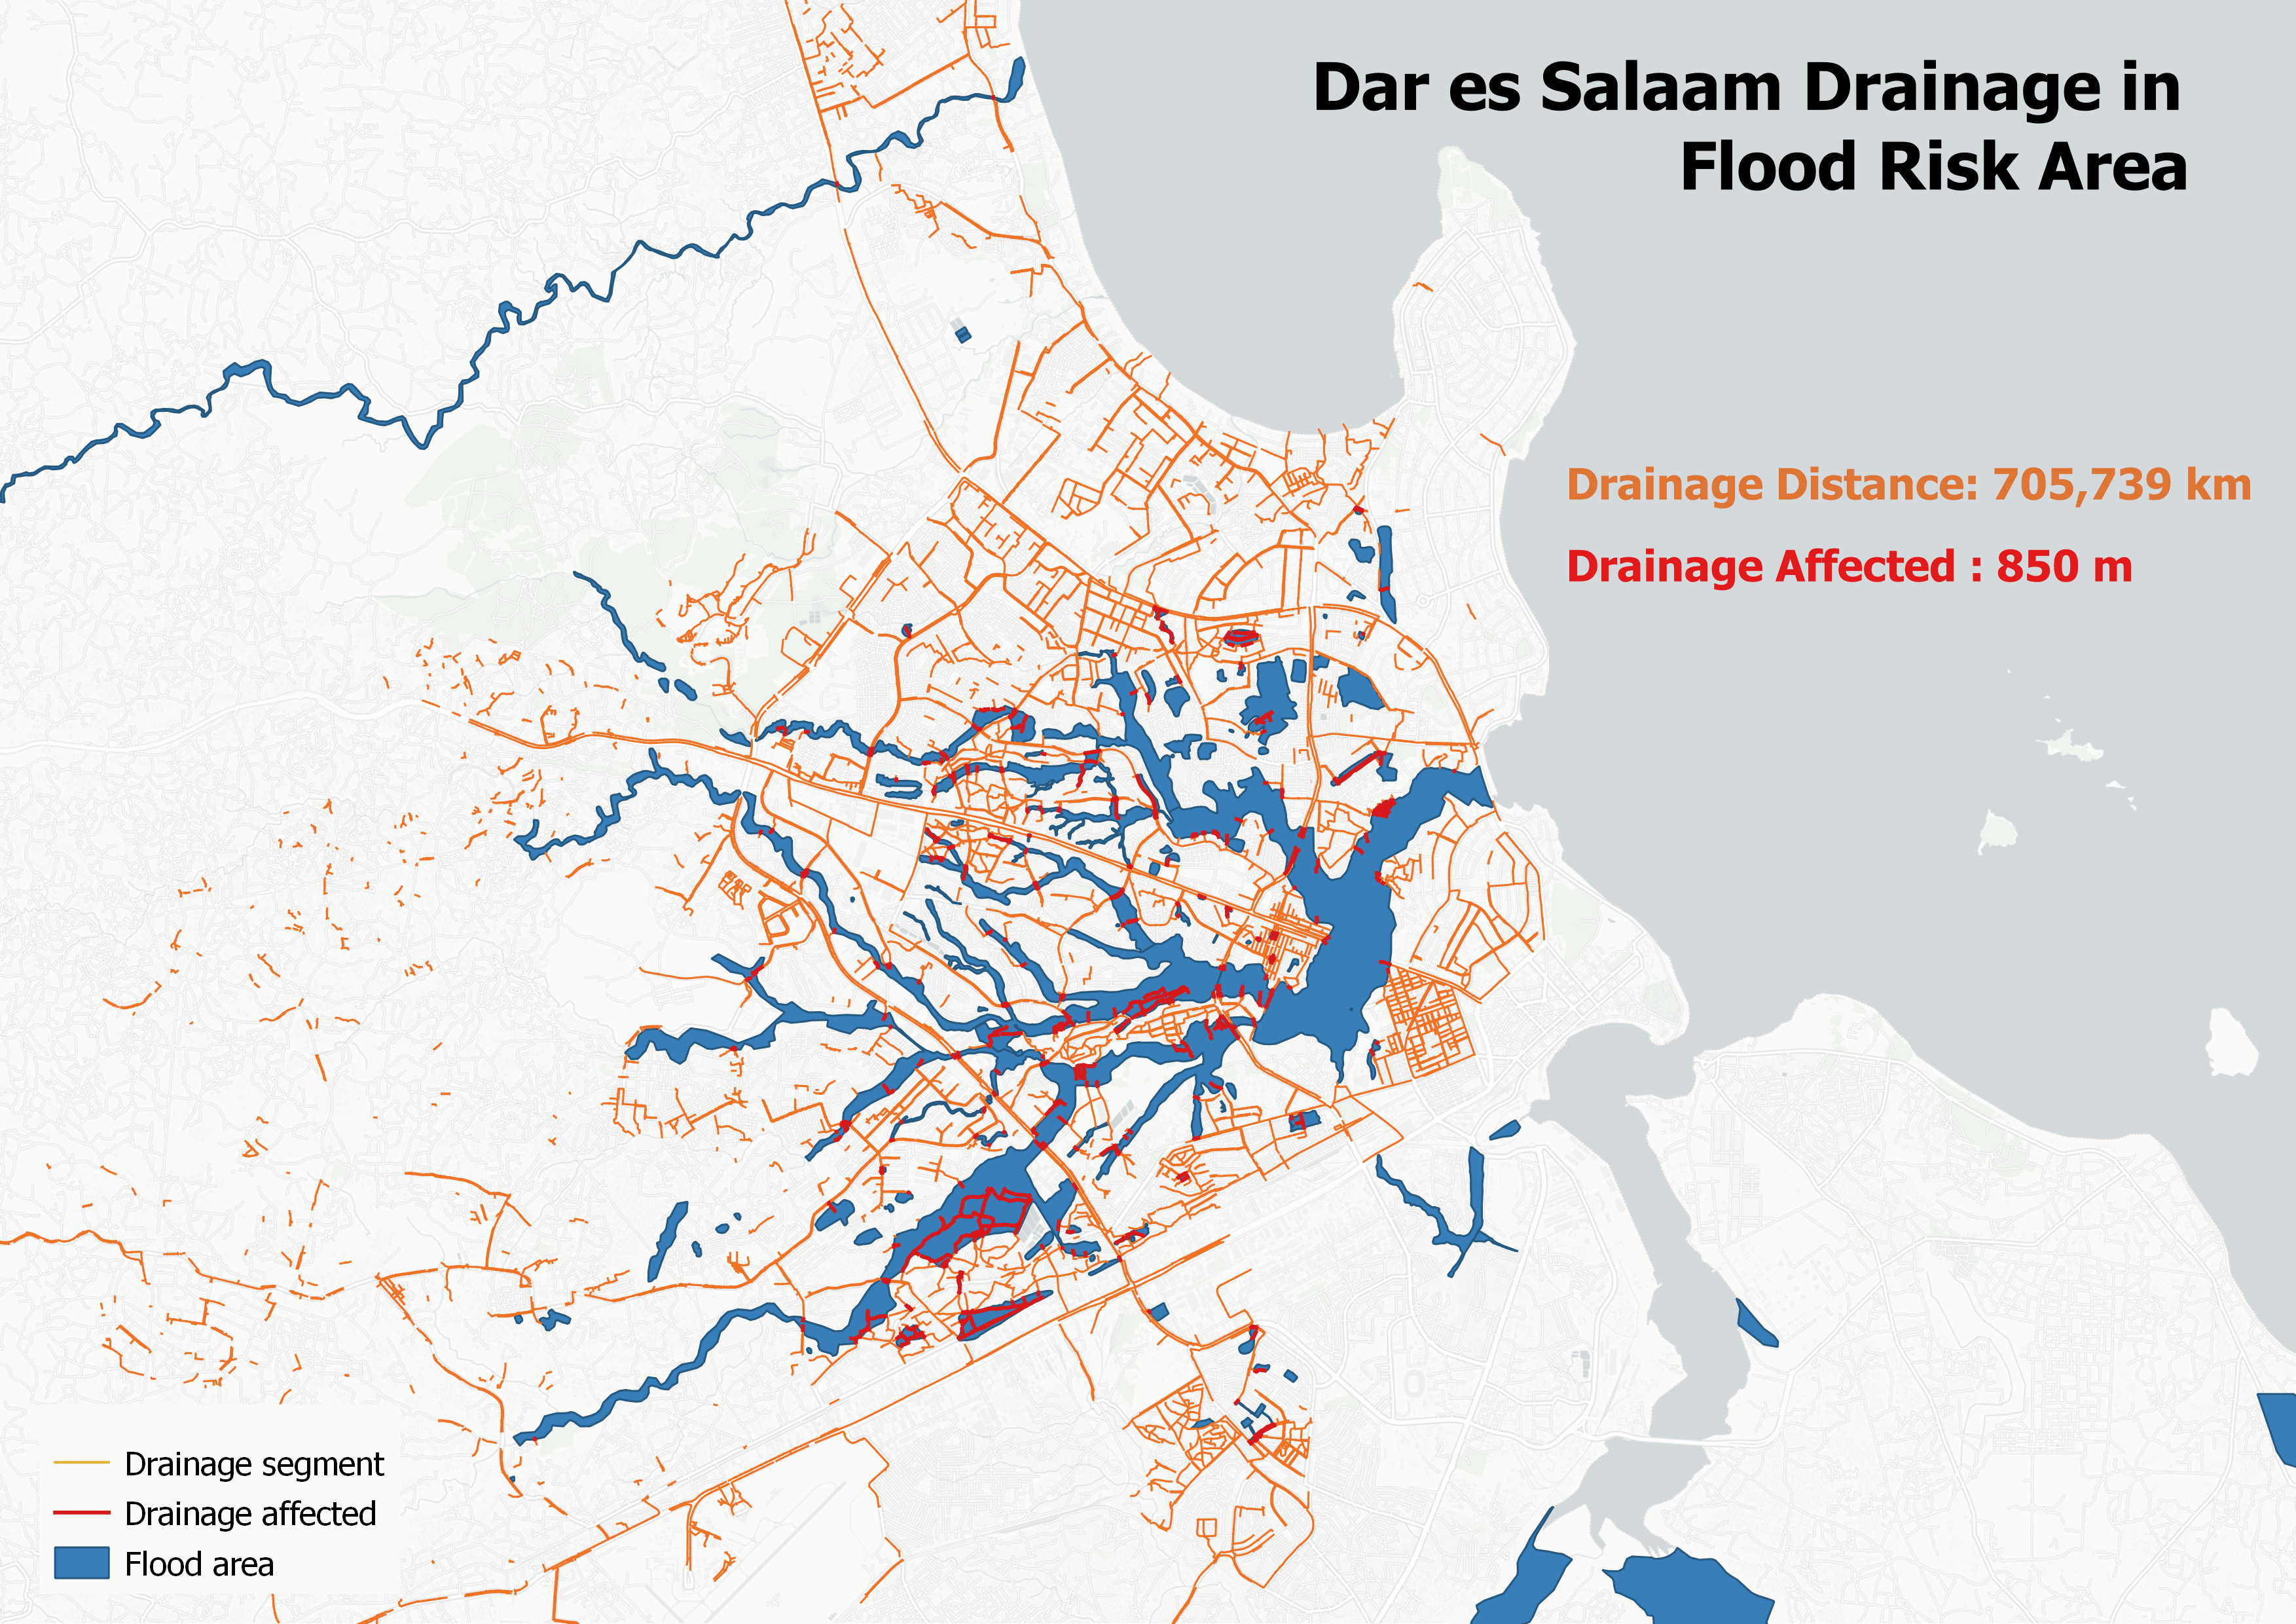
\includegraphics[width=.8\textwidth]{images/drainmap_min.png}
    %\caption{Caption}
    \label{fig:my_label}
\end{figure}
Drainage data was collected in the most flood-prone areas across Dar es Salaam using cheap and practical methods. This information will be used to develop a flood model that requires accurately collected specifications of drains such as depth, width, blockage (by either vegetation or material), connectivity, and diameter (typically for culverts). At the same time, the team worked with a hydrologist in Deltares, Netherlands, to finalize a tool for data quality checks (HydroOSM) which had a visible impact on our ability to collect high-quality data. 

18,350 segments of culverts, drains, ditches and decommissioned drainage infrastructure totaling 705 kilometers and 13,385 drain points including damage and blockage points, outflow, and points with no exit have been collected. A master’s student, Louise Peterson from TU Delft, concluded in her thesis that community mapped drainage data could improve flood prediction on a neighborhood scale.\footnote{ Community Mapping for Flood Modelling: A case study of the Ramani Huria community mapping project in Dar es Salaam, by Louise Peterson, 2019} This provides solid evidence for the power of the community approach, and that with training and practical experience students are able to achieve what was once the exclusive preserve of highly specialized professionals with expensive equipment. 

\newpage
\subsection{Community Assets and Threats Mapping}
\begin{figure}[h]
    \centering
    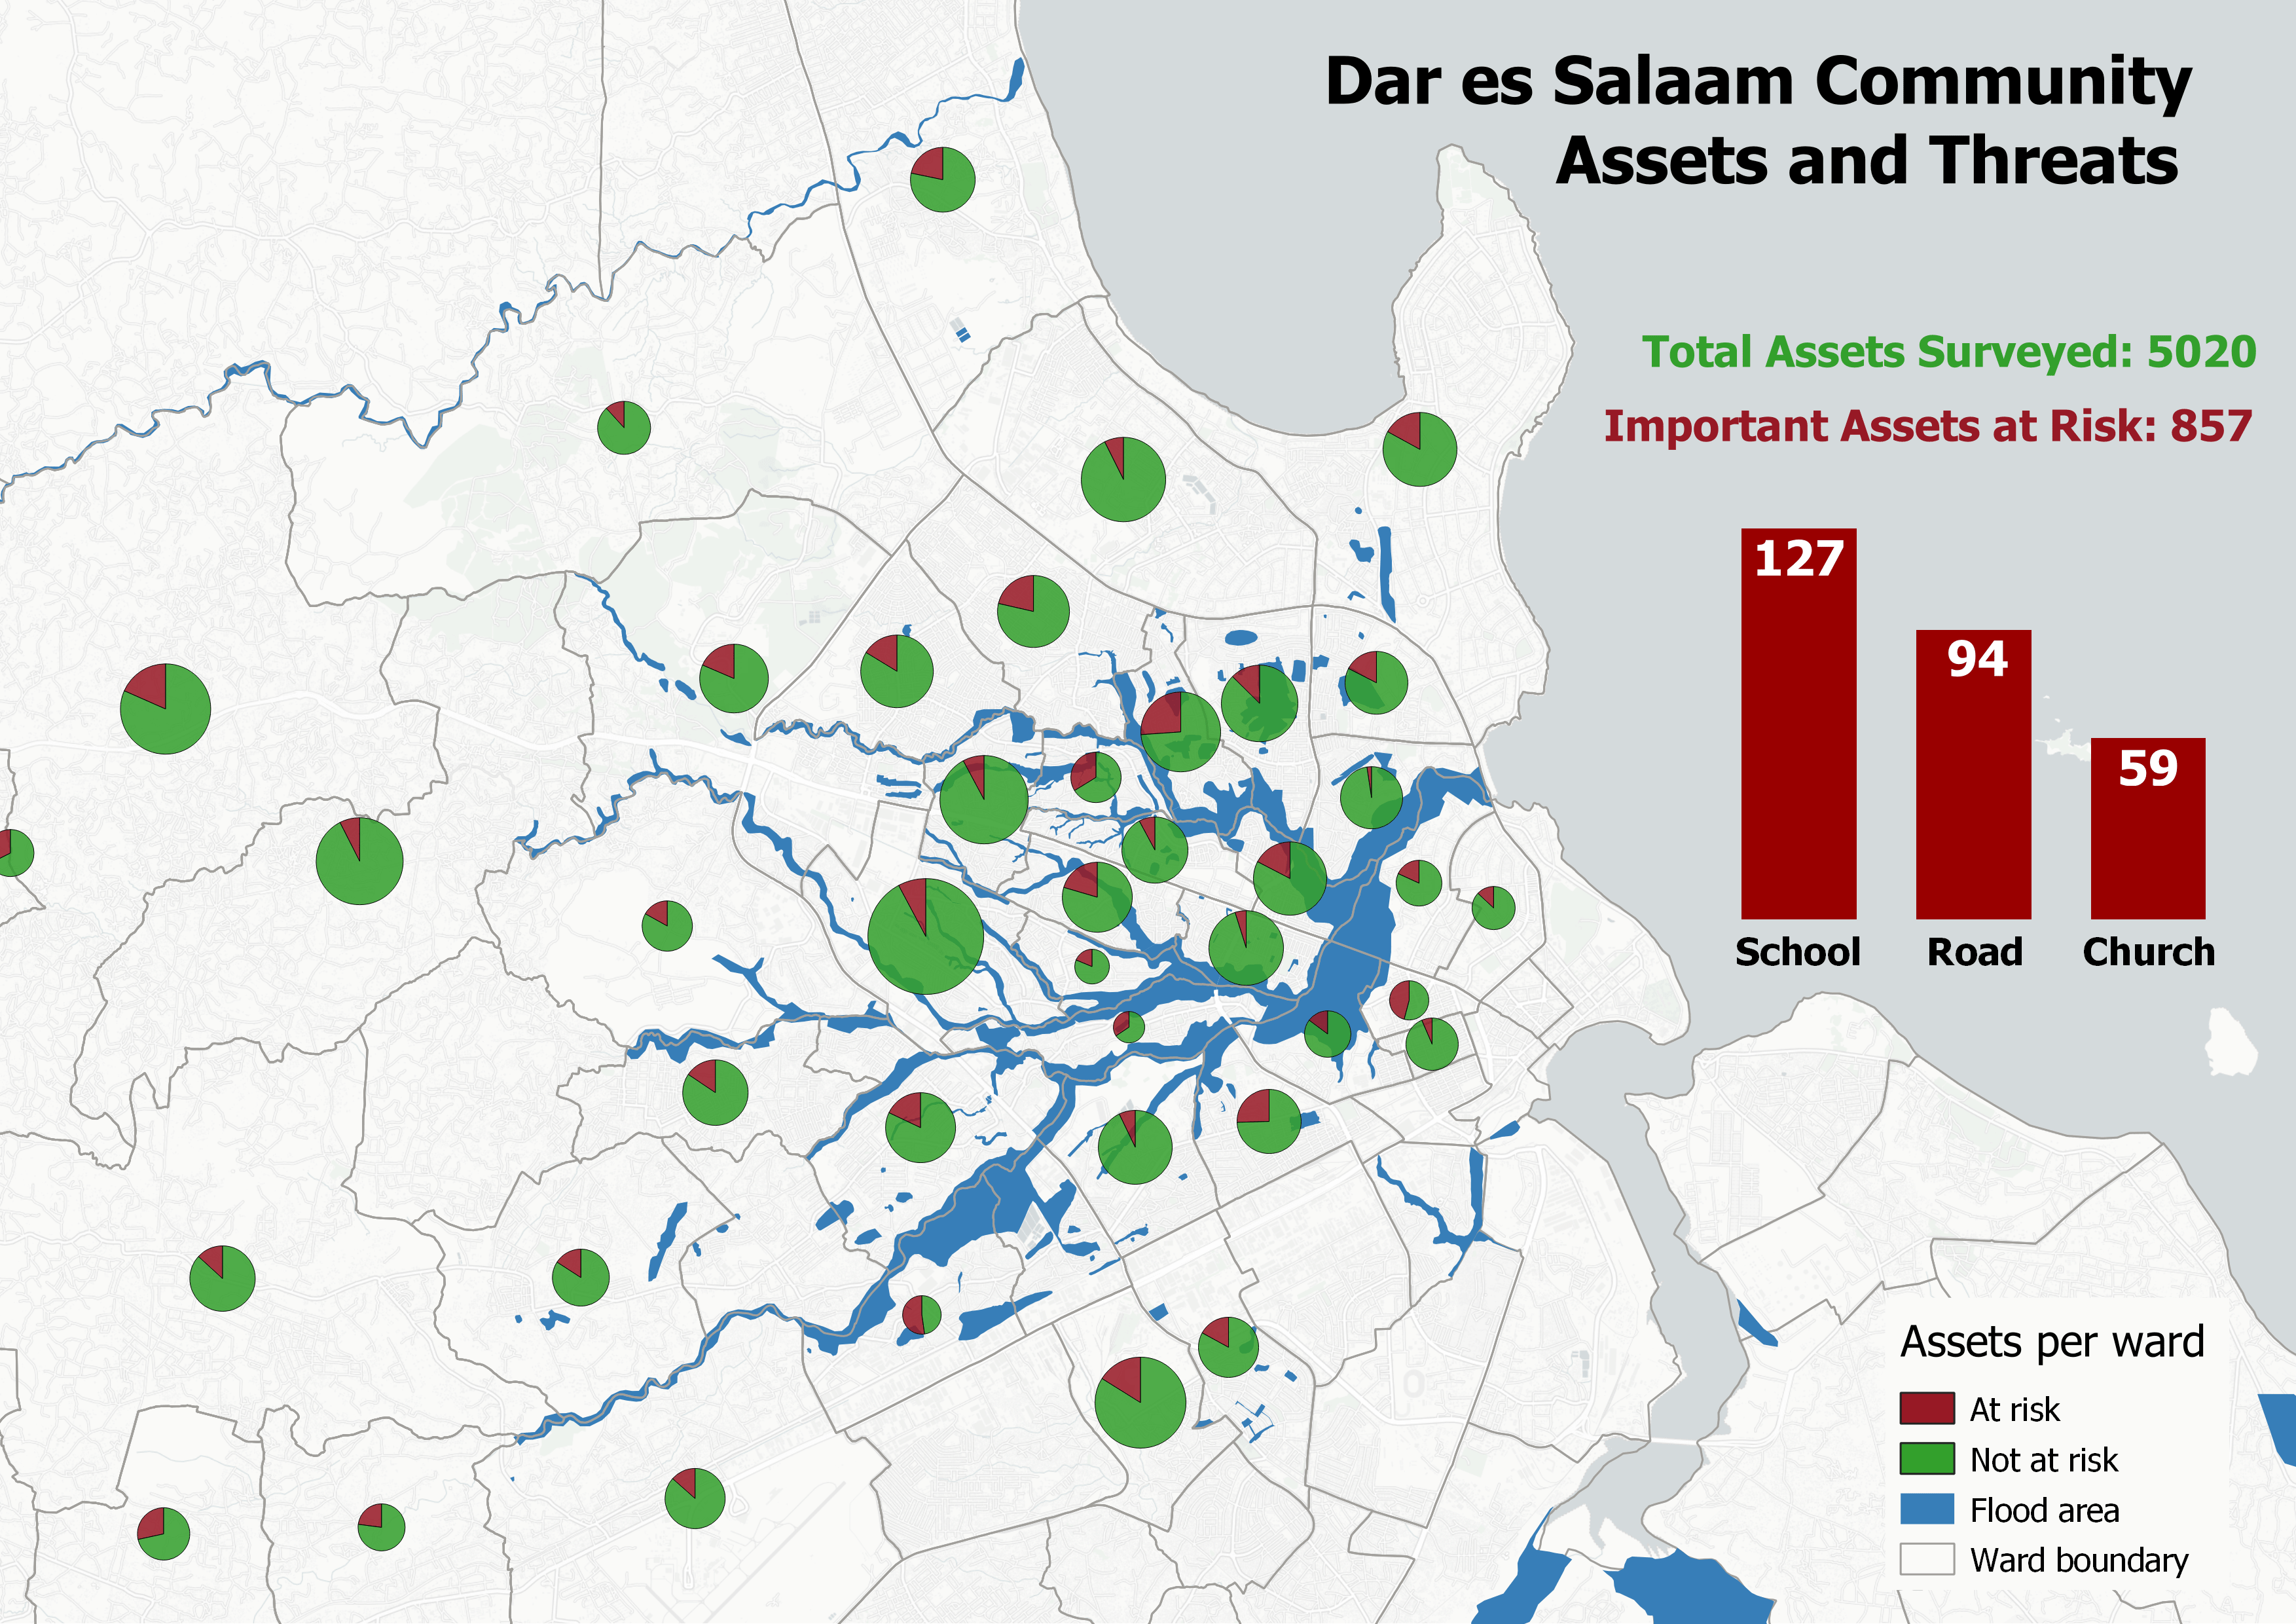
\includegraphics[width=.8\textwidth]{images/asset_pie_min.png}
    %\caption{Caption}
    \label{fig:my_label}
\end{figure}
Flood risk identification of flood-prone areas of the city was conducted through a series of meetings with influential community members and leaders to identify assets, threats, and evacuation centers and issues that contribute to flooding in their subwards. More than 5000 points including amenities that are affected and not affected by floods and evacuation centers were collected by students and community members during the 2017 Industrial Training.

In the project, assets were identified as amenities that are important to the community but not at risk of flooding, threats are amenities that the community thinks may flood if the hazard continues unabated and evacuation centers are areas that the community members affected by floods flee to for a safe stay. This information can only be provided by the community itself since they understand their neighborhoods better.

%\begin{centering}
%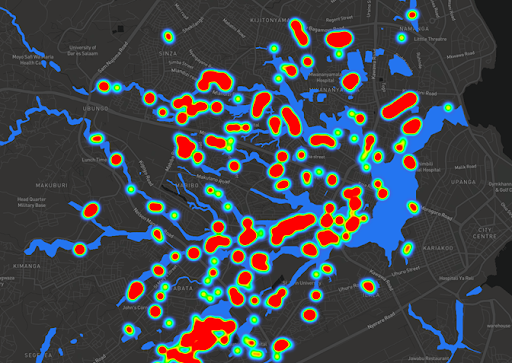
\includegraphics[width=\textwidth]{images/Asset_&_Threats_Viz.png}
%\end{centering}

\subsection{Trash Mapping in Dar es Salaam}
In collaboration with Nipe Fagio (“give me the broom” in Swahili), a civil society organization founded in 2013, Ramani Huria mapped trash sites in Dar es Salaam. The trash mapping initiative was part and parcel of the larger Let’s Do It World campaign, a civic-led mass movement to clean up countries.

9452 trash points were mapped and put into an interactive web map. The mapped data helped to identify the location of the areas with poorly managed waste materials, type and size of the waste and clean up methods. This process helped ease cleaning the city on September 15th, 2018, a celebration of World Clean-Up Day by mapping existing solid waste and assist solid waste contractors to improve their customer relationships by mapping clients systematically to the doorstep.

\subsection{Building Footprint Digitization}
Re-digitization of the city was conducted to update and improve the quality of already digitized layers using COWI imagery with 10cm resolution provided by the Ministry of Lands, Housing and Human Settlements. Previously the city was digitized using either Bing, Mapbox or Digitalglobe which have lower resolutions compared to COWI imagery.

Aligning buildings with a higher resolution image of 10cm provided by COWI company using Mbtiles created in GDAL (gdaladdo)---a utility used to build or rebuild overview images. Using the 2016 COWI imagery in combination with the HOT Tasking Manager, buildings were re-digitized in JOSM and validation of the re-digitization was done by the validation team.


\begin{figure}[h]
    \centering
    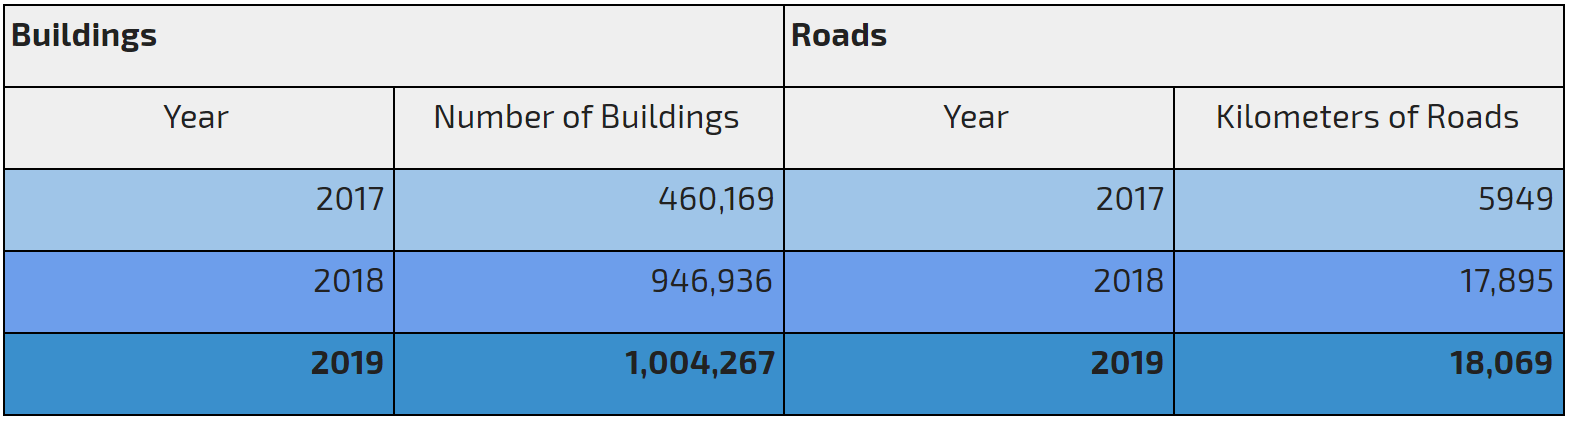
\includegraphics[width=\textwidth]{images/BuildingsAndRoads.PNG}
    \caption{The following table indicates the analytics of the buildings and roads mapped by the team during the Ramani Huria project timeline (2017/2019)}
    \label{fig:my_label}
\end{figure}
\newpage
\subsection{Hyperlocal Boundary Mapping}
\begin{figure}[h]
    \centering
    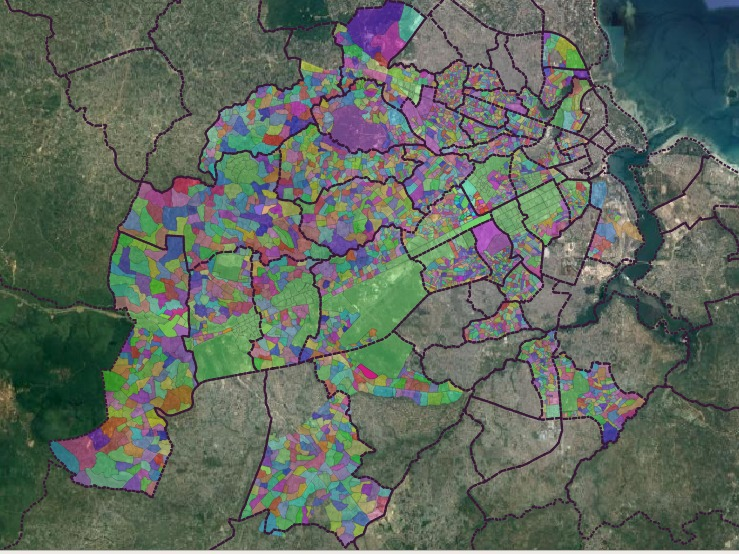
\includegraphics[width=.8\textwidth]{images/shinaexample.jpeg}
    %\caption{Caption}
    \label{fig:my_label}
\end{figure}

Hyperlocal boundaries, known locally as Shinas, are divisions within subwards regarded as political boundaries administered by local leaders (wajumbe). Previously referred to as Ten Cell divisions as they were originally comprised of ten households, these divisions now comprise of 30 to 200 households due to the increase in population. Wajumbe are increasingly functioning as non-partisan public servants, often the first point of interaction between the government and citizens.

Given the rate of urbanization in Dar es Salaam, it is very difficult to locate people and their respective addresses due to the unplanned and informal settlements nature of these communities. Using more granular boundaries, however, makes it easier to locate people and provide services more precisely. HOT was able to map more than 3000 hyperlocal boundaries in Dar es Salaam with the sole focus of incorporating a layer of health access information and issues to flood plans. This will better inform emergency responders and flood response plans. 

Amana Hospital in Dar es Salaam is now using the patient origin tracking system---electronic Health Information System (eHIS)---that was developed using data collected from the hyperlocal boundaries mapping as part of Ramani Huria. The data can also be used for disaster management and rescue i.e. fire or floods by Multi-agency emergency response teams, especially if the data is incorporated with highways.
\newpage
\subsection{Trash Mapping on Formal Settlements}
\begin{figure}[h]
    \centering
    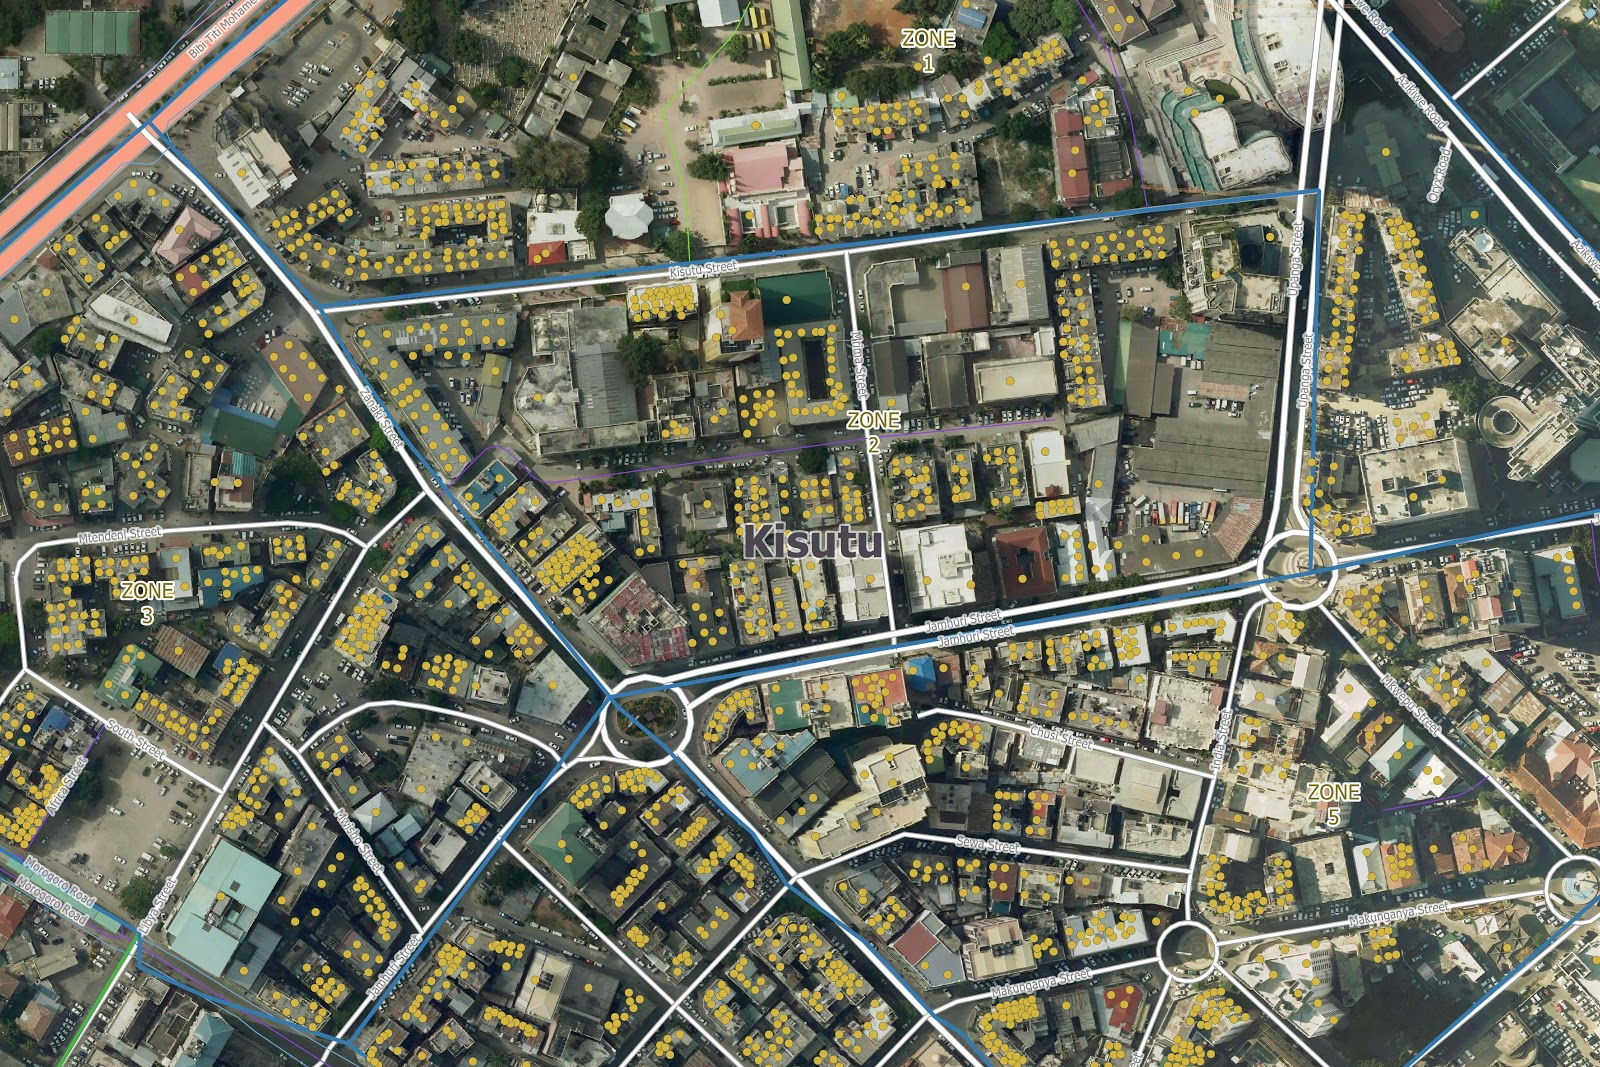
\includegraphics[width=.8\textwidth]{images/Trashmapsample.jpeg}
    %\caption{Caption}
    \label{fig:my_label}
\end{figure}

Ramani Huria and Green WastePro Ltd. (GWPL)---a private company specialized in waste management with the aim to offer eco-friendly solutions in cleaning and waste management---partnered in August 2018 to provide datasets for waste management. They mostly operate on formal settlements using robust barcode stickers developed specifically for their clients. The company needed a digital methodology to obtain clients’ information including locations, clients' contacts etc, so they can track clients and provide services accordingly. The HOT team collected building data for each structure (resident/client) using robust barcode stickers placed at each unit completing a survey gleaned along with some amenity information. 

A total of 4706 clients mapped and around 4500 client data points are used by the company to collect trash. The results show that simply knowing the location of clients creates a sustainable business model  for solid waste management companies in Dar es Salaam. 

\newpage
\subsection{Soil Sediment Sampling}

With the support of the World Bank in Tanzania, Ramani Huria and JBA Consulting partnered in October 2018 to develop a surface soil sediment dataset for the greater Dar es Salaam region of Tanzania. This was intended to support a geomorphological assessment taking into account soil sediment characteristics for erosion and flood risk studies.

A national-level soil profile had existed for Tanzania prior to this effort but contained only a single sample from Dar es Salaam. This was not sufficient to analyze erosion potential across the city. The JBA team in consultation with Ramani Huria decided to use a 2km grid, which resulted in 731 sampling points being pre-established throughout the city.

\begin{figure}[h]
    \centering
    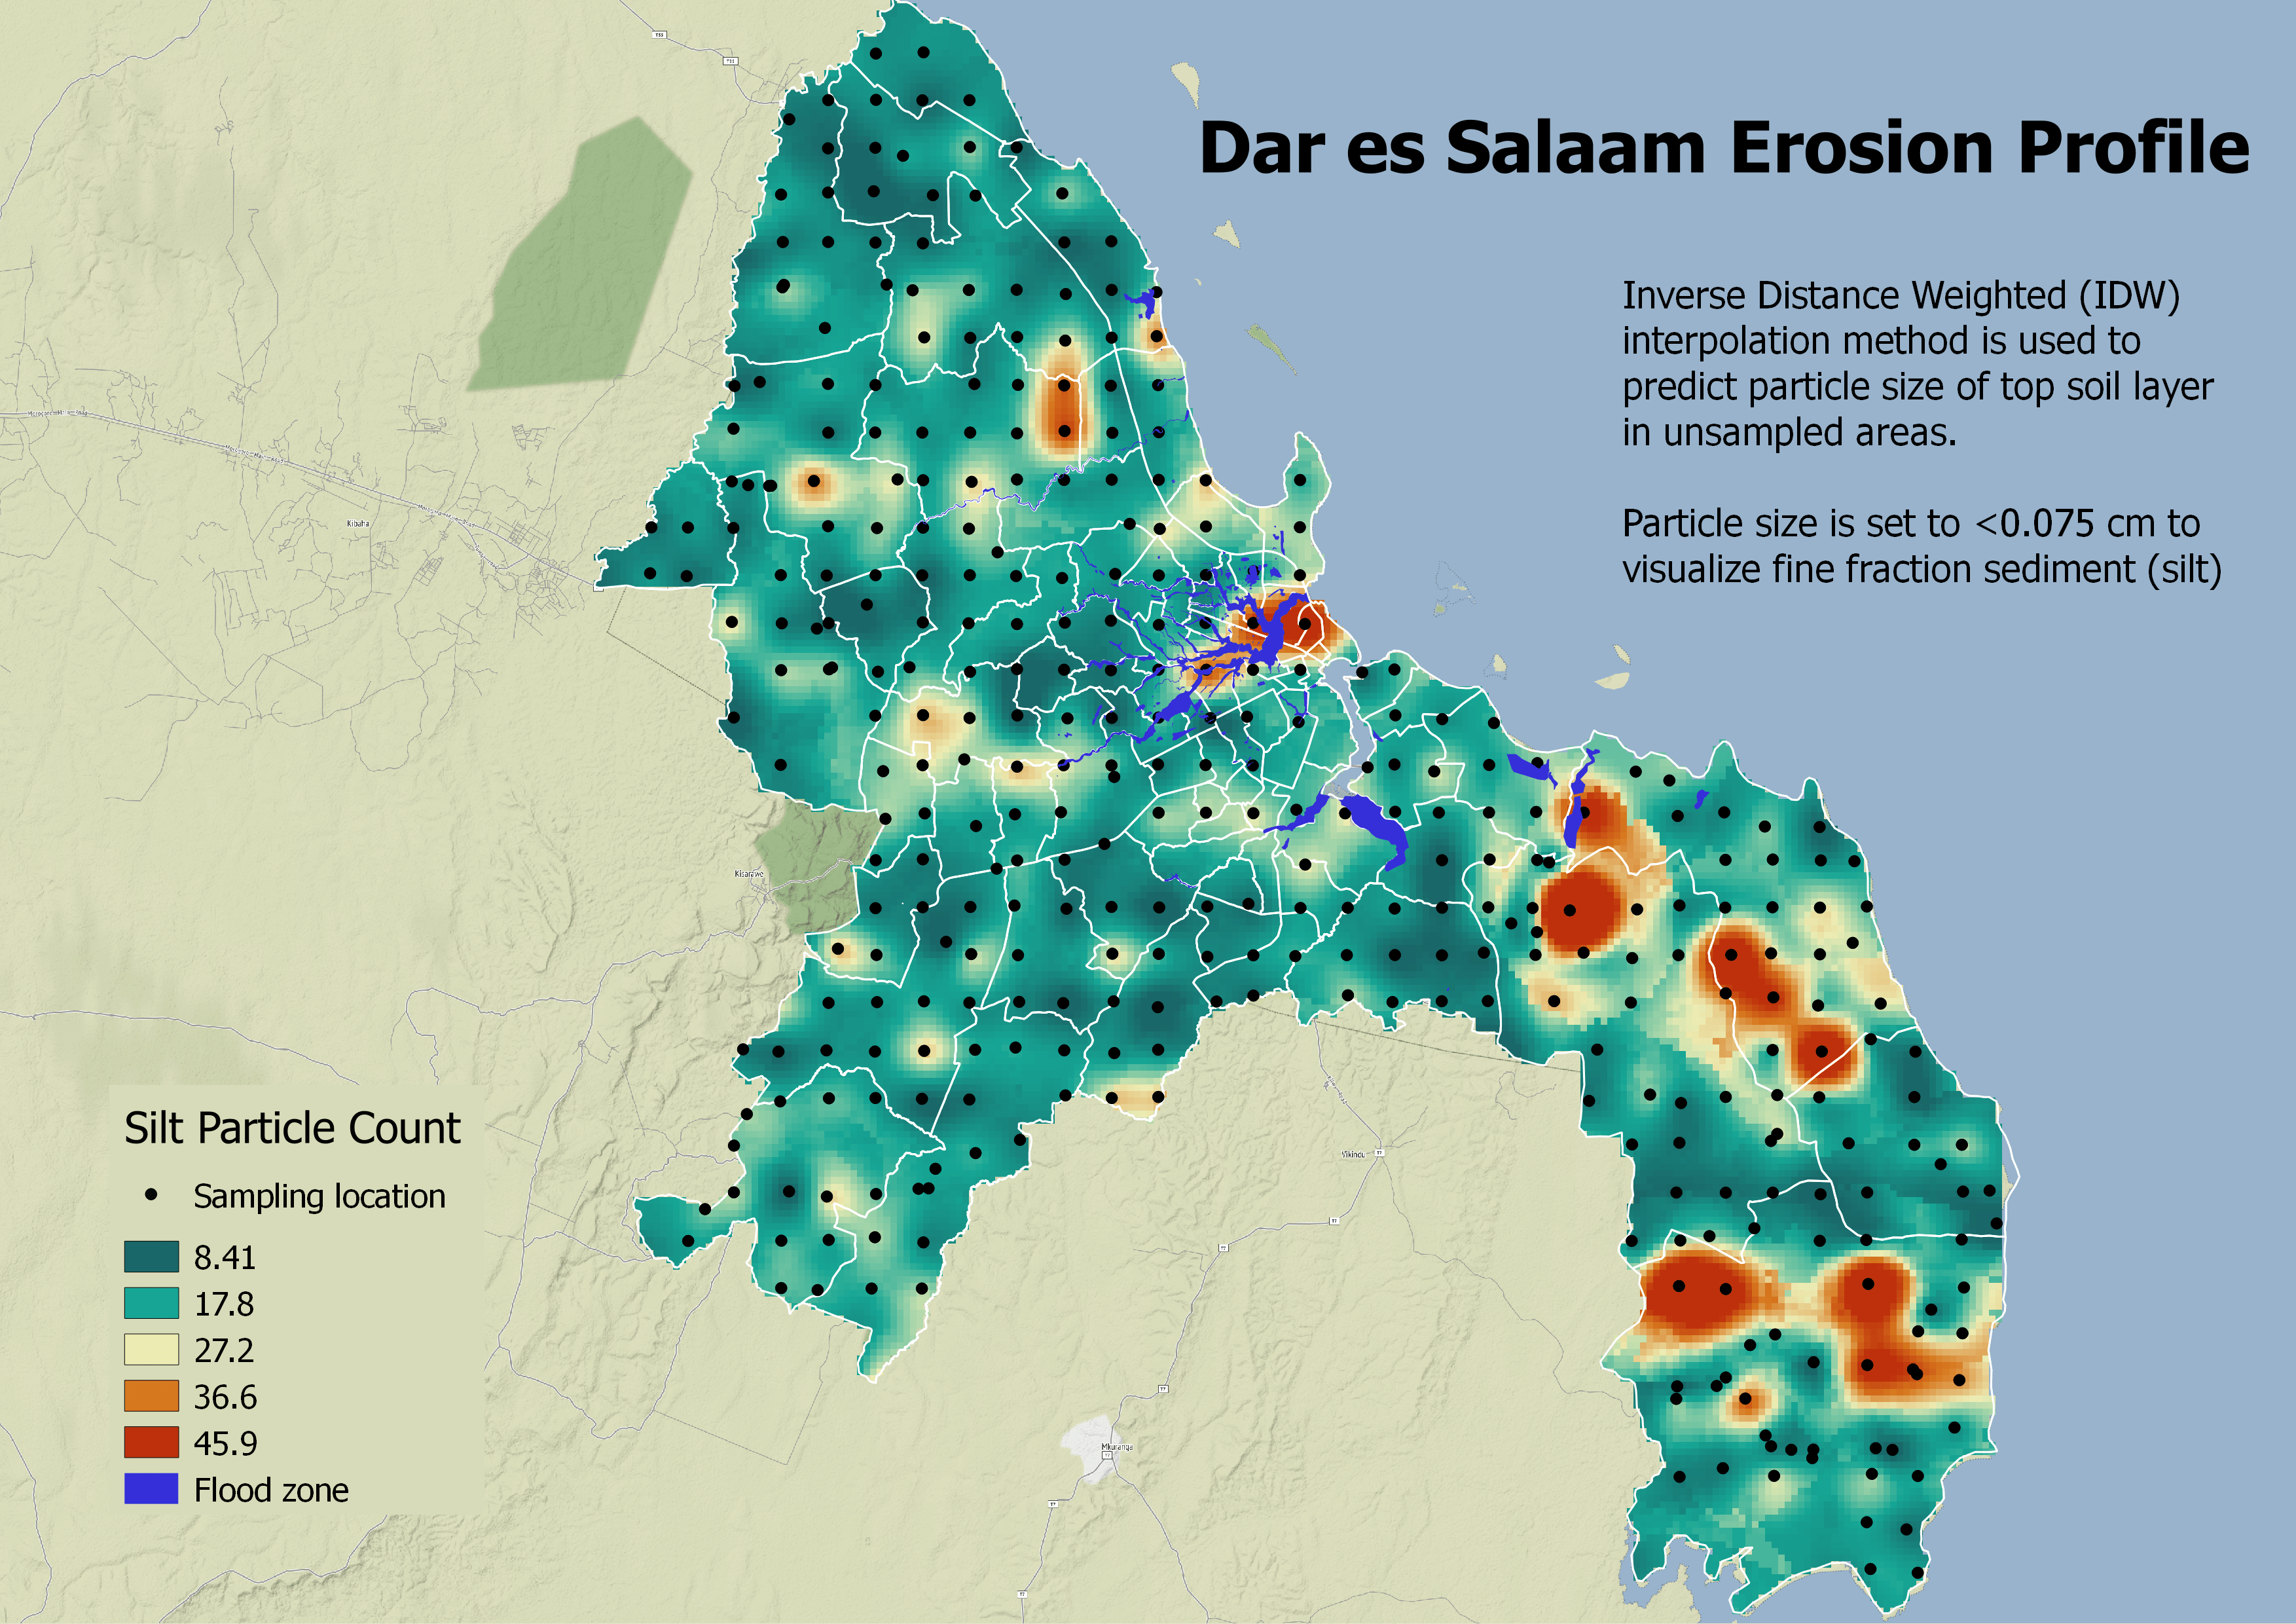
\includegraphics[width=.75\textwidth]{images/erosion_Sep26_min.png}
    %\caption{Caption}
    \label{fig:my_label}
\end{figure}

A total of 643 points were sampled and sieved; 88 sites were inaccessible or were hard to collect samples because they fell into paved areas, military bases, the ocean, etc. A detailed Soil Sediment Sampling wiki\footnote{\url{ https://wiki.openstreetmap.org/wiki/Soil_Sediment_Sampling}} was prepared by the HOT team explaining all the procedures that were conducted by the team to obtain sediment material from all over the city and some parts of the Pwani region.

Using particle size, the data will allow visualizing the spatial distribution of different types of surface and subsurface soils. For instance, the map below visualizes the spatial distribution of silt (particle size between 0.002 mm and 0.075 mm) using the Inverse Distance Weighted interpolation method. Thus, it helps identify areas that are suitable for agricultural planning and expansion. It also identifies areas that are suitable for agriculture but are at risk of being flooded. For more details, see the full soil sampling report, A Surface Soil Sediment Profile for Dar es
Salaam,Tanzania.\footnote{\url{https://github.com/ivangayton/soil-sampling-report/blob/master/Soil_Sediment_Sampling_Final_Report.pdf}}

%\in\in
\newpage
\setlength{\parskip}{0.7em}
\subsection{Community Flood Response}

\begin{figure}[h]
    \centering
    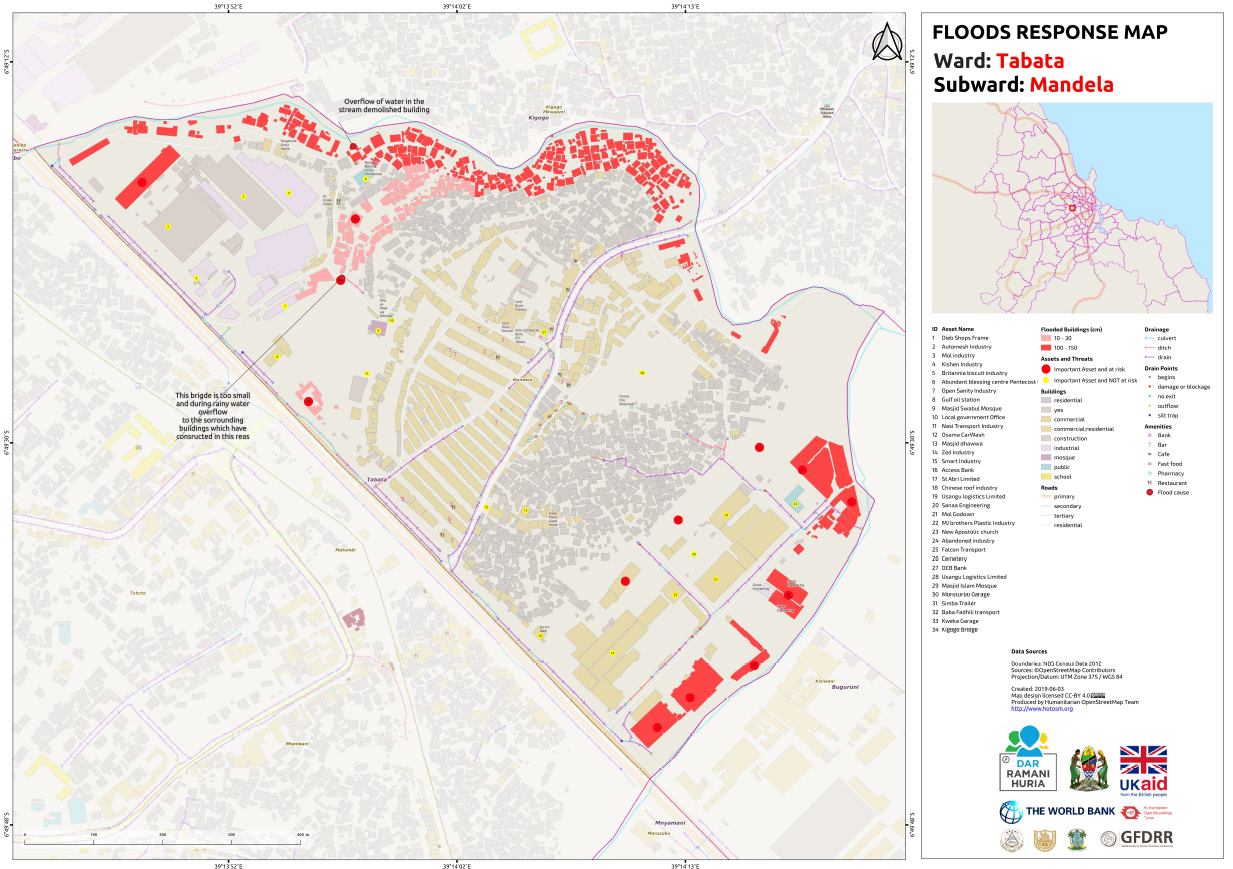
\includegraphics[width=.75\textwidth]{images/mandelaexample.PNG}
    %\caption{Caption}
    \label{fig:my_label}
\end{figure}

As a response to heavy rainfall in March and May 2019 which resulted to heavy flooding in some wards of Dar es Salaam, the Ramani Huria team conducted field mapping to engage affected communities with the aim of conducting a rapid assessment and producing impact maps. With reference to the past flood responses done in the city, the Ramani Huria team led the way to identify effects in the communities and create maps to help responders on the ground. The team responded by visiting flooded areas to assess the impact.

Through using our local leaders’ contact database that contains more than 3000 phone numbers, the team was able to contact these local leaders to remotely identify the subwards affected and the effects.
This information will be used to conduct a damage assessment of the affected areas. The data has been shared with the Red Cross, which will help them to prepare for the next rainy season and for risk prevention analysis.

\section{Best Practices and Lessons Learned}

%\begin{multicols}{2}

The Ramani Huria project, unlike many other projects that deal with data, focused on community participation guided by the principle of ‘Local people, local devices and open knowledge'. Meaning,  working with local people in Tanzania (community members, students) to add local knowledge to an open database using devices that are locally available and empowering students to use  their own smartphones as a key device in data collection. Under typical circumstances, a similar project might have hired professional engineers and data analytics to complete the work. However, as this project was based on a local capacity building, especially among university graduates, the focus on training local students and community members to complete the project was one of the major successes of the project.

Through the course of this project, academic institutions have turned to Ramani Huria for training and guidance on their curriculum. Professors from both Ardhi University and the University of Dar es Salaam have asked for—and received—training in GIS and data collection tools as well as support to use OpenDataKit (including Ramani Huria-derived improvements) for their projects. In addition to academic outreach, local businesses including ride-share companies, have sought out support in using the data for routing and other business development purposes. 

The project team utilized low-cost surveying drones to monitor specific infrastructure, river basins and even in response to flood situations. These drones, costing a few thousand dollars, can be deployed under the cloud cover with greater ease and higher frequency than more traditional surveying drones.   A local pilot has been trained as a result of the project and is in the process of developing a Tanzanian-made drone to further minimize the cost of acquiring images for different disaster responses and any other fields that need aerial images.
%\end{multicols}

\subsection{Lessons Learned}

\textbf{Budgeting time for seeking permissions:} A common challenge in these types of activities is seeking permission for doing what may be suspicious-looking activities (running around random areas of a major city with a shovel, walking around measuring drainage channels, going door to door asking for people’s information, etc.) In order to ensure that these activities can be carried out successfully and to ensure data quality, it is critical to follow protocol and allocate appropriate resources.


\textbf{Fieldwork outpacing data cleaning and analysis:} In some cases, we underestimated the resources needed and time allocated to conduct specific activities. For example, correction of methodology and data issues occurred later in the process than desired and in some cases would have required returning to the field to recollect data.   

\textbf{Constant updating of collected data:} Some of the data may be very dynamic, for example, drain blockage and damage in certain points can change over a day, building uses and structures change over time, updating road names using both local and official names. This dynamic needs to be accounted for when planning field data collection and validation. It also requires planning on how data points will be revisited and updated. 

\textbf{Clear piloting and training:} Effective training with examples and hands-on experience needs to be provided to mappers before field excursions to save time and costs during data collection.

\begin{mdframed}[hidealllines=true,backgroundcolor=RHgreen!10,innerleftmargin=6pt,innerrightmargin=6pt,leftmargin=-3pt,rightmargin=-3pt]
\textbf{Areas for Future Data Collection:}
As Ramani Huria comes to an end and is being taken forward by the Resilience Academy, the project team can provide guidance to the Academy in identifying areas that can be completed through future projects, such as those areas that were not able to be covered during the scope of this project.
\end{mdframed}

\section{Ongoing and Future Impacts}

Through the OpenStreetMap platform and partners such as the Resilience Academy, Ramani Huria data will continue to be maintained and updated to be used in development and economic decision-making long after the end of this project. Too often, quality data is collected but remains unused, whether due to lack of awareness or limited engagement and collaboration with stakeholders. Ramani Huria mitigated for these factors during project design and implementation to ensure continued support and use of the data by local partners. We did this by involving relevant stakeholders and beneficiaries of the project right from the beginning of the project, creating a sense of data ownership, which in turn will increase data use in the future.

We have already seen case studies of independent data use and applications giving us confidence that this data will continue to have an impact. As one example, in August 2015, the Tandale ward officer used Ramani Huria maps to locate the source of Cholera cases to determine the point of contamination. The maps provided them with detailed information on water points and sanitation data, thus allowing his team to investigate the sources of the outbreak, similar to the John Snow initiative in response to the 1859 Cholera outbreak in London. The following sections provide further examples of current and future impacts of Ramani Huria data. 

\subsection{Ongoing Impacts}

\begin{enumerate}
\item \textbf{Disaster Response Agencies:} Organizations are using maps and data to identify areas affected, conduct damage assessment and provision of relief to the victim. Decision-makers such as the Prime Minister's office, Dar es Salaam Metropolitan Development Project (DMDP) offices, and others through disaster departments can also use the data in disaster risk management plans to have a clear insight into cost analysis for risk response and preparedness.
\item \textbf{Emergency Response:} Services such as Fire, Red Cross, and DarMAERT, use the data in planning for disaster response as the data simplifies access to the affected areas. Much of this is attributed to Ramani Huria's mapping of roads and  providing street names, both local and official.
\item \textbf{Health sector:} Data collected through Ramani Huria is aiding assessments in the contingency of pandemic diseases, such as cholera, that occur during flooding. This data is being used to locate the geographic spread of the disease and identify the source of infection as well as track patient origin. This can be evidenced by \href{https://www.hotosm.org/updates/piloting-tanzanias-first-patient-origin-tracking-system/}{Tanzania’s First Patient Origin Tracking System}\footnote{\url{https://www.hotosm.org/updates/piloting-tanzanias-first-patient-origin-tracking-system/}} implemented at the Amana Regional Referral Hospital in Dar es Salaam.
\item \textbf{Companies:} Our methods of data collection are being used by local businesses to improve and run their companies. For example, Green Waste Pro LTD, a trash collection company in Dar es Salaam, worked with us to develop a dataset and a system to track and locate their clients for better service and revenue collection. The company’s revenue tripled as they started using our datasets. This is the result of the training and support they received from the Ramani Huria team.
\item \textbf{Government Institutions:} Through Ramani Huria training, government institutions are changing the way they operate and approach issues. As an example, the President's Office Regional Administration and Local Government offices (PORALG) is now working on administrative boundaries using our technical capabilities.
\item \textbf{Institutions/NGOs:} Through the influence of the Ramani Huria project, the development of technical and managerial skills in local staff has allowed for OpenMap Development Tanzania to be established and take on new projects. Other organizations such as Nipe Fagio (\textit{"Give me the broom"} in Swahili) are using Ramani Huria data to strengthen their cleaning operations in the city.
\item \textbf{Development Actors:} Organizations such as Palladium now look to Ramani Huria for a wide range of technical expertise. GIZ, the German Development Agency, collaborated with the Ramani Huria team to better understand and work with industrial actors in riparian areas. In another case, Ramani Huria staff performed soil sampling to improve erosion modeling in the city, including the actual sample analysis and interactive map data visualization to improve solid waste management governance.   


\end{enumerate}

\subsection{Potential Future Impacts}

Datasets, maps, tools, learning materials, and documentation will be carried on and used by the Resilience Academy as well as other interested companies, institutions or organizations. Based on the past and ongoing use cases of Ramani Huria tools, data, and methodology, we anticipate a broad range of future impacts as stakeholders develop new ideas and continue integrating methodology and data into their practices. 

\begin{enumerate}
    
\item \textbf{Urban planning:} The Ramani Huria basemap data is more accurate and up-to-date than typical information available in most of local councils. This data will help decision-makers with urban planning issues, such as urbanisation and gaps in services.
\item \textbf{Local Government Authorities and the communities:} Having a clear insight into the risks in their surroundings with map data will be critical  to creating plans for mitigation such as fixing blocked drains, trash management, etc.
\item \textbf{Academic institutions, Non-Governmental Organizations, and Companies:} Organizations and institutions can use collected data as evidence and supporting documentation to design future projects, providing services (i.e rescue activities during flooding or other hazards). We also anticipate this data being used in business and economic development by businesses relying on location and navigation data (i.e. Uber and Taxify).
\item \textbf{Transportation:} Routing and network analysis i.e bus routing, delivery services, aid logistics, and resource allocation for hospitals and dispensaries can be conducted using mapped data.

\end{enumerate}

\section{Legacy: Tools, Processes, and Capacities}

Ramani Huria did not just collect data. Rather, it created a way to collect the data, provided guidelines, and transferred knowledge to those who will carry this forward. The people who have gained these skills and knowledge have the capacity to train other cities and countries who would wish to replicate the project. Among others, Ramani Huria will leave a legacy in the following key aspects:
\begin{enumerate}
    \item Ramani Huria has created an apprenticeship system for students, allowing students to learn by doing and participating in real project activities in the field. Through this system, a number of graduates who participated in the project are now implementing different projects with the technical and managerial capacities to run even larger projects in the future.
    \item The knowledge gained by students and community members throughout the implementation of the project will increase the use of data produced and contributing to creating a resilient city with a strong, young and enthusiastic community that believes in data-driven policies and decisions. Knowledge and understanding of the data will also be a good start to inform other decisions that were not the primary goal of the project---making the data even more valuable as it will be used to inform multiple decisions such as in health systems, planning, and infrastructural development.
    \item Having detailed datasets in one of the fastest growing and unplanned cities is a big step towards creating a better sustaining and resilient city. For this reason, other countries are looking towards Ramani Huria as a model for using community mapping for urban resilience. In this way, the project impact has gone far beyond Dar es Salaam and can even be named as  ‘the largest community mapping initiative in Africa’ serving as a community-mapping model for other African countries and worldwide. Other countries like Zambia, Mozambique, Sierra Leone are now looking back at the project and see the potential of replicating it.

\end{enumerate}

\subsection{Communications and Media Coverage}

Effectively communicating the goals, progress, and potential data use has been critical for the success and impact of Ramani Huria. The project has been covered by both local and international media, which is key to disseminating its values and ideas. Through our social media platforms (Facebook, Instagram, Twitter), blogs on our website, as well as direct contacts with people at conferences, gatherings, and workshops, we have managed to reach a significant number of individuals, organizations, and communities. 

Due to dedicated communications and outreach efforts, we have been contacted by a number of media outlets, such as the BBC, to conduct interviews about the project; volunteers who connected with us through social media and dedicated their time to work with us for free; students from different universities who wanted to do their research and thesis based on the project; and students interested in using the project for practical training.

%\bigskip


%%\begin{tabular}{|c|c|c|c|}
%\hline
 %%S/N & Video & Description  \\
% \hline 
%%1 & \href{https://www.youtube.com/watch?v=VtDcR_e8_vQ}{Ramani Huria Project 2.0} \footnote{\url{https://www.youtube.com/watch?v=VtDcR_e8_vQ}}    & The launch video of Ramani Huria 2.0, building on the pilot\\ 
%{} & {} & done from 2015-2016.\\
%%\hline
%2 &  \href{https://www.youtube.com/playlis%t?list=PLb9506_-6FMEcMtUtvJV1bKOrW89HNFMd}%{HOT Tanzania %Playlist}\footnote{\url{https://www.youtub%e.com/playlist?list=PLb9506_-6FMEcMtUtvJV1%%bKOrW89HNFMd}} & A playlist of ten videos %showcasing Ramani Huria\\
%{} & {} & and different activities in Dar %es Salaam\\
%\hline
%3 & \href{https://www.youtube.com/watch?v=%7Pa0wgMstE8}{Ramani Huria -}\\ 
%%{} & Community Mapping in Dar es salaam\\
%\footnote{\url{https://www.youtube.com/wat%ch?v=7Pa0wgMstE8}}
%\end{tabular}


\subsubsection{Videos Featuring the Project}
\bigskip
\begin{itemize}
    \item \href{https://www.youtube.com/watch?v=VtDcR_e8_vQ}{Ramani Huria Project 2.0} \footnote{\url{https://www.youtube.com/watch?v=VtDcR_e8_vQ}}
- The launch video of Ramani Huria 2.0, building on the pilot done from 2015-2016.
    \item \href{https://www.youtube.com/playlist?list=PLb9506_-6FMEcMtUtvJV1bKOrW89HNFMd}{HOT Tanzania Playlist}\footnote{\url{https://www.youtube.com/playlist?list=PLb9506_-6FMEcMtUtvJV1bKOrW89HNFMd}}
- A playlist of ten videos showcasing Ramani Huria and different activities in Dar es Salaam
    \item \href{https://www.youtube.com/watch?v=7Pa0wgMstE8}{Ramani Huria - Community Mapping in Dar es Salaam} \footnote{\url{https://www.youtube.com/watch?v=7Pa0wgMstE8}} - Tanzanians are mapping their own city in order to solve flooding using better urban planning, better drainage and maintenance and better community waste management.
    \item \href{https://www.worldbank.org/en/news/video/2019/05/15/in-tanzania-citizen-scientists-help-reduce-flood-risk-with-soil-sampling}{In Tanzania, Citizen Scientists Help Reduce Flood Risk with Soil Sampling}\footnote{\url{https://www.worldbank.org/en/news/video/2019/05/15/in-tanzania-citizen-scientists-help-reduce-flood-risk-with-soil-sampling}}
- The Tanzania Urban Resilience Program harnessed local tools and knowledge to create a comprehensive soil map that will inform flood mitigation measures and urban planning for the city of Dar es Salaam
    \item \href{https://www.youtube.com/watch?v=6-hKycm9oOY}{How Tanzanians are Mapping their own City to Solve Flooding}\footnote{\url{https://www.youtube.com/watch?v=6-hKycm9oOY}}
- As a community-based mapping project in Dar es Salaam training university students and local community members to create highly accurate maps of the most flood-prone areas in the city, Ramani Huria is helping Tanzanians to map their own city in order to solve the problem of flooding using better urban planning, drainage and maintenance, and community waste management.
    \item \href{https://www.youtube.com/watch?v=920-Uuzlais}{Data and Drones Combat Flooding}\footnote{\url{https://www.youtube.com/watch?v=920-Uuzlais}}
- Everyone is impacted by the effects of flooding in Dar. Armed with handheld global positioning system (GPS) units and drones, a team of university students and community members is determined to change that by gathering data to promote flood resilience.
    \item \href{https://youtu.be/Y77bwq8XnJM?t=4}{ Data for Waste Collection (Swahili)}\footnote{\url{https://youtu.be/Y77bwq8XnJM?t=4}}
How can technology contribute to clean Dar es Salaam? Azam Tv which is one of the famous local television networks featured Ramani Huria work about data produced for trash collection companies to track their clients
\end{itemize}

\subsubsection{Radio}
\begin{itemize}
    \item \href{https://www.bbc.co.uk/programmes/w3cswgqx}{Mapping Africa's Megacities.} \footnote{\url{https://www.bbc.co.uk/programmes/w3cswgqx}}
- Katie Prescott of BBC reports from Dar es Salaam, Tanzania's most populous city. Its population is growing at more than 4 percent every year, often with little planning. The slums of the  Kigogo district, for example, are regularly inundated by the neighboring rivers, as community leader Osiligi Losai explains.
\end{itemize}

\subsubsection {Blogs/Articles}

\begin{itemize}
    \item \href{https://www.thecitizen.co.tz/magazine/success/-Local-graduate-using-drones-for-mapping/1843788-4967500-c6pj0rz/index.html}{Local Graduate Using Drones for Mapping}\footnote{\url{https://www.thecitizen.co.tz/magazine/success/-Local-graduate-using-drones-for-mapping/1843788-4967500-c6pj0rz/index.html}}
- How a local graduate (Bornlove Ntikha) built a drone from scratch after joining the Ramani Huria team as a student mapper.
    \item \href{https://www.ippmedia.com/en/features/hot-tackles-dar-es-salaamE28099s-waste-problem-one-dataset-time}{Tackling Dar es Salaam’s Waste Problem - One Dataset at a Time} \footnote{\url{https://www.ippmedia.com/en/features/hot-tackles-dar-es-salaamE28099s-waste-problem-one-dataset-time}}
- Through the project, we have worked with trash collection companies to better understand their challenges and found a better way to track their clients by location, know their number and create a better system of revenue collection.
    \item \href{https://spectrum.ieee.org/robotics/drones/tanzanias-homegrown-drone-industry-takes-off-on-bamboo-wings}{ Tanzania Builds a Drone Industry From Local Know-How and Bamboo}\footnote{\url{https://spectrum.ieee.org/robotics/drones/tanzanias-homegrown-drone-industry-takes-off-on-bamboo-wings}}
- Bamboo drones are just one way that local companies hope to meet Tanzania’s needs. Bornlove Ntikha uses bamboo for the frame of his DIY drone. Ntikha wants to show that drones can be built out of locally available materials, which will make them cheaper and more accessible.
\end{itemize}

More Blogs about the project are found on \href{http://ramanihuria.org/news/}{Ramani Huria Website}\footnote{\url{http://ramanihuria.org/news/}}. The blogs include both technical parts of the project and data use.

\newpage
\section{Conclusion: From Local to Global Solutions}
\begin{multicols}{2}

The Ramani Huria project set out to prove that local people, equipped with local devices and open knowledge, can provide data for urban resilience that is fit for purpose in ways that traditional "professional" providers and methods cannot. 

At the heart of this is \textit{inclusion}. If local people are involved in the conversation about resilience---and they understand and have ownership of the goals---they can contribute in ways that not only equal but surpass the output of traditional data systems. Local people must be more than an inexpensive labor force; to reach their full potential they must be genuine partners in the enterprise of building more resilient cities.

Local people, local devices, and open knowledge are not limited by expertise and equipment from abroad, or from proprietary licenses, and the cost of local salaries and transportation is orders of magnitude smaller than that of experts from abroad. Local people can create data---and impact---on the vast scale needed to keep up with the urban growth of places like Dar es Salaam.

The data, processes, documentation, and knowledge created by Ramani Huria is a tremendous legacy for the city of Dar es Salaam. However, the key resource is the people. Hundreds of students and thousands of community members have learned not only \textit{how} to collect data, but \textit{why} to do so. A small but significant number---perhaps a dozen or so---Ramani Huria participants are now recognized, despite being in their twenties, as leaders and experts in urban resilience. Their own former university professors, government departments such as the PO-RALG and TAMISEMI, NGOs and donors such as Palladium and PATH, private businesses like Green Waste Pro and other waste entrepreneurs call upon these Ramani Huria alumni for not only their expertise, but also their ability to understand real problems and conceptualize effective solutions. 

The best of the Ramani Huria participants don't just do as they are told, they seek out problems that matter to them, their peers, and their city. They imagine solutions. They fail. They learn from failure and try again. They persist. Ultimately they create solutions both rooted in the lived experience of native Tanzanians and empowered by the vast open knowledge of the global commons. 

They pass their knowledge to their peers unstintingly, secure in their competence and unafraid of competition. They welcome, rather than fear, more people being able to do what they can---they are aware of the tremendous amount of work that remains to be done for resilient cities. 

Several Ramani Huria alumni are already engaged in supporting projects across Africa and beyond. More will fly like seeds from a great flowering tree, creating new teams and projects across Tanzania and beyond. The fundamental power of local people, local devices, and open knowledge has revolutionized urban resilience data in Dar es Salaam. The world is watching, and the work is only beginning across the globe.


\end{multicols}

\newpage
\section{Glossary}

\textbf{Java OpenStreetMap Editor (JOSM):} JOSM is an extensible editor for ​OpenStreetMap (OSM). It supports loading GPX tracks, background imagery, and OSM data from local sources as well as from online sources and allows to edit the OSM data (nodes, ways, and relations) and their metadata tags.


\textbf{Mjumbe (Wajumbe):} These are community appointed leaders to administer a shina in a subward. Mjumbe (plural ‘Wajumbe’) is the main, trusted point of contact for local households over issues such as public services, resource allocation, and community pain points. They’re chosen by their community to act as their representative to the government and to relay government decisions and initiatives back to the community (such as waste collection processes).


\textbf {OpenDataKit:} is a free and open-source set of tools for collecting data and fill out a  survey. It's been used to collect billions of data points in challenging environments around the world. ODK Aggregate is a Java server that stores, analyzes, and presents survey data collected using ODK Collect.


\textbf{OpenMapKit:} OpenMapKit (OMK) is an extension of OpenDataKit allowing users to create professional-quality mobile data collection surveys for field data collection. OpenMapKit launches directly from OpenDataKit when the OSM question type is enabled in a standard survey. Simply include OSM questions and tags in your survey to collect information on OSM in the field.


\textbf{PORALG:} President's Office Regional Administration and Local Government offices. The ministry coordinates rural and urban development management policies and strategies.


\textbf{Shinas:} These are sometimes also referred to as “ten-cell units”, since originally these areas were meant to cover ten households. Now, due to population growth, a shina tends to contain between 30 and 200 households. Each shina is administered by a ‘mjumbe’.

\section{Annexes}
\href{https://wiki.openstreetmap.org/wiki/Dar_es_Salaam/Ramani_Huria}{Ramani Huria Data Model}

\href{https://drive.google.com/file/d/1M0jcJHxdIDlrCRr09c4G8ZVlvl43j_1b/view}{Ramani Huria Cookbook}

\href{https://docs.google.com/document/d/1PwHRtdRvOfeEhpsIl-gpQXTTDoVwW_0--wRsmeUhVt4/edit#}{Inception Report}

\href{https://docs.google.com/document/d/1oW4y4ZT76viHu_sDnrBYrFsJfu_a0CAn9GLIxmG_rpc/edit}{1st Interim Report}

\href{https://docs.google.com/document/d/1Zn35NGLn2n-X93Z2hwiWwQwUnMljCoD7hwTUrTEXxTg/edit}{2nd Interim Report}

\href{https://docs.google.com/document/d/1D03BG5Pkmo0XMIyrvvgVLqdeyfkmwxRRs3UQdekNspk/edit}{3rd Interim Report}

\href{https://docs.google.com/document/d/1Cc-ztcmc53LqlqhAXC1neCyxuRJujN16nhcibMg04qw/edit}{Technical Overview of Digital Assets}

Disaster Risk Reduction Plan Toolkit



























\end{document}